\documentclass[a4paper,11pt,oneside]{book} 
\usepackage{CS_report}
\usepackage{newfloat}

\DeclareFloatingEnvironment[fileext=loe, listname={List of Equations}, name=Equation]{myequation}

\begin{document}
    \captionsetup[figure]{margin=1.5cm,font=small,name={Figure},labelsep=colon}
    \captionsetup[table]{margin=1.5cm,font=small,name={Table},labelsep=colon}
    
    \frontmatter    
    \begin{titlepage}      
        \begin{center}
            \includegraphics[width=6cm]{figures/lumen_logo.png}\\[0.5cm]
            {\LARGE Lumen Data Science\\[0.5cm]
           Team: MedMax}\\[2cm]

            \linespread{1.2}\huge {
                Project documentation
            }
            \linespread{1}~\\[2cm]
            {\Large Haralović Marko} \\ [0.001cm] 
            {\Large Štolfa Duje}\\[1cm] 

            {\large 
            A project documentation submitted as part of the solution for the Lumen Data Science task in year 2024./2025.} \\ 
            {\large April 2025}          
        \end{center}
    \end{titlepage}

    \tableofcontents
    \listoffigures
    \listoftables
    \listofmyequation

    \mainmatter
    \chapter{Business understanding}
\label{ch:business_understanding}

\section{Melanoma diagnostic process}
Melanoma is a malignant tumor caused by the uncontrolled division of pigment-producing cells called melanocytes. These cells are mostly contained in the epidermis, the outermost layer of skin, so the greater part of melanoma cases are skin cancer, with rare occurrences in the retina or mucosal surfaces \cite{visual_inspection}. Malignant melanocytes become dangerous when they start spreading to deeper layers of skin, from where they can enter the blood stream and lymphatic system, and rapidly metastasize to any part of the body. Because of this, melanoma are responsible for the majority of skin cancer deaths, even thought they are not the most common type of skin cancer \cite{cnn_vs_derm}. 
This makes early detection of melanoma a critical aspect in ensuring full patient recovery.

The diagnostic process for melanoma can involve a lot of clinical examinations, but the final decision comes down to a dermatologist who has to decide whether to biopsy a given lesion or not \cite{visual_inspection}. This examination is done visually, typically using a dermatoscope, a tool that magnifies the lesion, reduces reflections and increases the visibility of some features of the lesion and the skin around it. Here, the criteria that clinicians use to asses whether or not a lesion is suspected to be malignant have evolved over time, and range from a few simple rules that can even be used by the patients themselves, to analytically identifying complex lesion structures and analysing the individual's clinical history and risk factors. Some commonly used malignancy criteria include:

\begin{itemize}
    \item ABCD(E) warning signs \cite{abcde}
    \begin{itemize}
        \item Any lesion that has an uneven shape (A, asymmetrical), irregular edges (B, border), multiple colors within it (C), is larger than 6mm in diameter (D), and changes over time (E, evolution) is possibly malignant
        \item Simple and typically used by non-experts, without using a dermoscope
        \item It does not account for features that are typical for nodular melanoma
    \end{itemize}
    \item Seven-point checklist \cite{seven_point}
    \begin{itemize}
        \item Used to assess changes in size, shape, color, sensory changes, the presence of inflammation, crusting/bleeding and a diameter larger than 7 mm
    \end{itemize}
    \item Three-point checklist \cite{three_point}
    \begin{itemize}
        \item A lesion is likely to be malignant if it has any two of the three criteria
        \item The criteria are (1) asymmetry of color and structure (not necessarily shape), (2) the presence of an atypical pigment network (holes or lines), or (3) any type of blue-white color
        \item Requires the use of a dermatoscope
    \end{itemize}
    \item Pattern analysis \cite{pattern_analysis}
    \begin{itemize}
        \item This criterion involves identifying both global patterns and local features, and matching them with the specific structures and patterns that are typical for either malignant or benign lesions
        \item A dermatoscope is required to be able to see the fine structures in the lesion
    \end{itemize}
    \item Ugly duckling sign \cite{ugly_duckling, isic_2020_dataset}
    \begin{itemize}
        \item Highlights the importance of clinical context in the diagnostic process
        \item When making a diagnosis, the decision if one lesion is atypical is made based on other lesions on that same patient
        \item If a lesion is considered to be atypical (the "ugly duckling") for that specific patient, it has a high chance of being malignant
    \end{itemize}  
\end{itemize}

Given that a referral to a specialist can take a substantial amount of time, and that melanoma can progress very rapidly, urgent reactions made by general practice clinicians could mean the difference between a quick recovery from a small biopsy and multiple years of recovery from metastasized tumors. This is where a reliable technological solution could step into play and aid the decision-making process of not only general practice clinicians, but also expert dermatologists. Developing any technological solution that is to be used in real-world clinical contexts is a big responsibility, and a necessary condition for the deployment of that system is its high reliability. The following sections go over the theory behind the process of ensuring this reliability in the development of a system for melanoma detection.

\section{Fairness of ML systems}

Technological systems aside, unjust treatment of social groups has been an ubiquitous problem in various aspects of human work both now and in the past. A lot of effort is currently being put into the active mitigation of discrimination and any kind of prejudice that could lead to it. To be able to assess fairness and mitigate biases, it is useful to detect which groups of people are going to be affected by the product or process we are designing, and what are the unintended consequences or harms going to be for them. This approach to fairness is commonly known as group fairness, and the characteristics based on which we define these groups are called sensitive features (e.g. gender, race, income).

\subsection{Types of harms}

Harms can be very diverse, and in any particular case we can be dealing with multiple types of harms at the same time. A few common types of harms include the following \cite{fairlearn}:

\begin{itemize}
    \item Allocation harms
    \begin{itemize}
        \item A system under- or over-allocates resources, opportunities or information
        \item e.g. consistently not approving a personal loan to a group of people who would have managed to pay it back (wouldn't default on the loan)
    \end{itemize}
    \item Quality-of-service harms
    \begin{itemize}
        \item The performance of a system is not equal across groups
        \item e.g. a voice recognition system that is less accurate when presented with non-native accents
    \end{itemize}
    \item Stereotyping harms
    \begin{itemize}
        \item The system perpetuates stereotypes
        \item Both positive and negative stereotypes can be harmful
        \item Most commonly, autocompletion software in search engines produce stereotyping harms
    \end{itemize}
    \item Quality-of-service harms
    \begin{itemize}
        \item A system behaves as if a certain group or some characteristic attributes of a person don't exist
        \item e.g. an application about the history of DNA research does not include any information about the work of Rosalind Franklin
    \end{itemize}
\end{itemize}

\subsection{Parity constraints and disparity metrics}

Identifying harms is a critical step in fairness assessment because all further analysis is then done with respect to the identified types of harms. Most importantly for machine learning systems, this lets us define appropriate measures of fairness. In the case of group fairness, these measures are based on requirements that a given model should perform comparably well across our relevant groups. These requirements are called parity constraints, and the corresponding measures of how well a certain parity constraint is satisfied are disparity metrics \cite{fairlearn}. 

For classification tasks, the most common and relevant parity constraints are demographic parity, equalized odds and equal opportunity. Achieving demographic parity should be prioritized if allocation harms are the most critical type of harm in a given domain. However, that system can still have varying false positive rates across groups and not have equitable accuracy. Thus, if both quality-of-service and allocation harms are important, we should aim at satisfying equalized odds. Equal opportunity also helps diagnose both allocation and quality of service harms, but is a relaxed version of equalized odds \cite{fairlearn}. Disparity metrics are discussed in more detail in chapter \ref{ch:evaluation} and are defined as either the maximum difference or minimum ratio between appropriate per-group performance metrics.

\subsection{The task at hand}

In the case of melanoma classification, we previously discussed that misdiagnosing a malignant lesion as benign means that that patient will not get the appropriate treatment, which could lead to severe consequences. On the other hand, the opposite case of classifying a dermoscopic image of a benign lesion as malignant only means that that person will go through further unnecessary medical examinations which will reveal that the initial diagnosis was falsely positive. In other words, false negative results translate to the under-allocated treatments and diagnoses. Knowing this, we conclude that allocation harms are more severe than quality-of-service harms, and satisfying demographic parity should be prioritized. 
    \chapter{Data understanding}
\label{ch:data_understanding}

\section{ISIC 2020 challenge dataset}
The ISIC 2020 Challenge Dataset \cite{isic_2020_dataset} is a publicly available collection of dermoscopic images accompanied by detailed metadata. The dataset includes 33,126 annotated training examples and 10,982 test images without annotations. These images depict skin lesions from over 2,000 patients, with both malignant and benign cases represented.

The dataset was curated for the SIIM-ISIC Melanoma Classification Challenge, hosted on Kaggle during the summer of 2020.

A notable limitation of the dataset is its strong tendency to underrepresent darker skin types. This imbalance can be attributed to unequal access to healthcare across populations and societal structures that affect which groups are more likely to be represented. As a result, any solution developed using this dataset is at risk of suffering from skin color bias. While this bias may seem expected given the data, it is a serious challenge from a modeling perspective. If our goal is to develop a truly generalizable solution, we must ensure that it performs equitably across all skin color groups; in other words, that it is fair.

Although the dataset is enriched for melanoma cases and does not reflect the true incidence of melanoma in the general population \cite{isic_2020_dataset}, it also exhibits a significant class imbalance between benign and malignant examples. This presents a major issue, the remedies for which we will discuss in later Chapters \ref{ch:data_preparation}, \ref{ch:modeling}.

The authors of the dataset \cite{isic_2020_dataset} also point out inconsistencies in lighting conditions across images. This variation can lead to inaccurate skin color estimation. If our only goal were to classify malignant lesions without concern for fairness, this might not be a critical issue. However, since we aim to develop a model that is not only high-performing but also fair, our modeling pipeline includes a skin color estimation component, making us directly affected by these inconsistencies.

In our modeling process, we do not use any metadata. We do not incorporate metadata into our knowledge base, nor do we train our models using both images and metadata, and our solution expects only images as input. More details are provided in Chapter~\ref{ch:modeling}.

\section{Skin color estimation}
Skin color is rarely annotated in publicly available dermatological datasets, with only a handful of datasets having labels for either the subject's ethnicity or the actual skin color \cite{skin_color_labels}. Additionally, as skin tone can be difficult to measure and quantify, researchers have not come to a consensus on which scale to use. Research in the makeup industry, for example, saw a need for a fine-grained scale like the L'Oréal skin color map \cite{loreal_chart, accel_fairness}. Medical researchers, on the other hand, needed a scale that reflects the effects ultraviolet light has on different skin tones, so they categorized skin types into the six Fitzpatrick skin phototypes \cite{fitzy} based on how likely each type is to burn or tan when exposed to UV light. Although this scale is completely subjective and is highly biased towards lighter skin tones because of its original application, it is commonly used in research, even when the use case is unrelated with the subject's reactiveness to sunlight. Because of this, we opt to use the individual topology angle (ITA) as a more objective and continuous measure of skin tone. 

\subsection{ITA estimation}
The first step of our data preparation and analysis was to estimate the subject's ITA for each image in the dataset. Following the procedure described in \cite{skin_color_bias_ferit}, we first mask out any pixels that don't contain skin (hair, lesions) and then cluster the remaining pixels to determine the dominant (most populous cluster) skin color in the image. If we represent the resulting color in the CIELAB colorspace, ITA can be estimated from its lightness $L$ and blue-yellow $b$ components. The detailed procedure is visualized in Figure \ref{fig:skin_segmentation} and is also documented in the  \lstinline{notebooks/skin_tone_estimation.ipynb} notebook. In summary, the segmentation procedure is based on image processing and includes increasing contrast with CLAHE, hair removal using DullRazor \cite{dullrazor} and morphologically expanded Otsu thresholding to remove skin pigmentations. 

\begin{figure}[p]
     \centering
     \begin{subfigure}{0.45\textwidth}
         \centering
         \includegraphics[width=\textwidth]{figures/estimation/estimation_A.png}
         \caption{}
         \label{fig:ss_1}
		 \vspace{0.5em}
     \end{subfigure}
     \hfill
     \begin{subfigure}{0.45\textwidth}
         \centering
         \includegraphics[width=\textwidth]{figures/estimation/estimation_B.png}
         \caption{}
         \label{fig:ss_2}
		\vspace{0.5em}
     \end{subfigure}
    \hfill
     \begin{subfigure}{0.90\textwidth}
         \centering
         \includegraphics[width=\textwidth]{figures/estimation/estimation_C.png}
         \caption{}
         \label{fig:ss_3}
		 \vspace{0.5em}
     \end{subfigure}
     \hfill
     \begin{subfigure}{0.45\textwidth}
         \centering
         \includegraphics[width=\textwidth]{figures/estimation/estimation_D.png}
         \caption{}
         \label{fig:ss_4}
		 \vspace{0.5em}
     \end{subfigure}
     \hfill
     \begin{subfigure}{0.45\textwidth}
         \centering
         \includegraphics[width=\textwidth]{figures/estimation/estimation_E.png}
         \caption{}
         \label{fig:ss_5}
		 \vspace{0.5em}
     \end{subfigure}
     \hfill
     \begin{subfigure}{0.90\textwidth}
         \centering
         \includegraphics[width=\textwidth]{figures/estimation/estimation_F.png}
         \caption{}
         \label{fig:ss_5}
		 \vspace{0.5em}
     \end{subfigure}
     \hfill
	\caption{Individual steps and results of the skin segmentation and color estimation procedure.}
	\label{fig:skin_segmentation}
\end{figure}

\begin{table}[]
\centering
\caption{Skin groups based on individual topology angle values from \cite{chardon}}
\label{tab:ita_ranges}
\begin{tabular}{lr}
\toprule
\textbf{ITA skin group} & \textbf{ITA range}  \\ \midrule
Very light              & $ > 55 $              \\
Light                   & $ \left<41, 55\right]$ \\
Intermediate            & $ \left<28, 41\right]$ \\
Tan                     & $ \left<-30.10\right]$ \\
Brown                   & $ \left<10, 28\right]$ \\
Dark                    & $ \le -30 $           \\ \bottomrule
\end{tabular}
\end{table}


Continuous skin tone labels like ITA enable us to test for correlations with continuous outputs of our model (e.g. prosterior probabilities of the malignant class) and in general contain more information than discrete skin tone types. Despite this, the task at hand is a classification one and our target variables are discrete (benign, malignant), so most fairness assessment techniques will require our data to be grouped based on skin tone. Because of this we discretize ITA into the six groups proposed in \cite{chardon}, shown in Table \ref{tab:ita_ranges}. As argued by \cite{letter_ita_fp} and as we previously hinted, we emphasize that these groups are not equivalent to the six Fitzpatrick phototypes which are more subjective and based on sun reactiveness of the subject's skin.

Figure \ref{fig:kde} shows the KDE plots of estimated ITA values for malignant and benign classes in the available dataset (aggregated training and validation sets of ISIC2020). It is evident that the dataset is biased towards lighter skin tones, especially in the benign case. The distribution of malignant ITAs is slightly wider, and its mean is shifted slightly more towards darker skin tones. Looking at skin color distributions with respect to the discrete ITA groups (Figure \ref{fig:histograms}), we notice that our dataset has no samples in the dark group, and that there are only two malignant samples in the brown group. These histograms show that, in addition to being imbalanced with respect to skin tone, our dataset is highly skewed towards the benign class. Most notably, malignant samples only make up $1.3 \%$ of the intermediate skin tone group. This is not surprising, as positive samples are bound to come up less often than negative ones when collecting dermoscopic or medical data. We see that our dataset is imbalanced in two orthogonal directions: with respect to skin color and malignancy. This is important to keep in mind in further analysis to be able to select appropriate classification models and methods.

\begin{figure}[htpb]
     \centering
     \includegraphics[width=0.8\textwidth]{figures/eda/kde.png}
     \caption{Per class individual topogy angle distributions in the available data.}
     \label{fig:kde}
\end{figure}
\begin{figure}[htpb]
     \centering
     \includegraphics[width=\textwidth]{figures/eda/histograms.png}
     \caption{Number of images in each skin color group for benign and malignant classes.}
     \label{fig:histograms}
 \end{figure}

\subsection{Estimation error checking}
Because we are doing automatic skin color estimation, we want to manually check for errors in the estimation results, and make sure that the estimated skin tones match our expectations for each group. Appendix \ref{ap:skin_color} shows 64 images from each skin color group, along with the estimated ITA values and corresponding dominant skin colors. With lighter skin tones and small lesions, the estimation appears to work correctly, and there is no need for corrections. We find that a lot of images which are classified as brown are heavily cropped and only show the lesion, with the surrounding skin being barely visible. In some of those cases we see that the skin color is actually much lighter than the predicted dominant one, and that the estimation was incorrect. 

Focusing only on the malignant samples in the brown and tan groups (Figure \ref{fig:ita_errors}), five mislabelled samples (marked in red) can be seen. These labels were corrected by taking the average RGB value in a 5x5 px area that was manually selected to only contain skin, and converting them to the CIELAB colorspace to calculate the corresponding ITA. The corrected skin tone labels are compared to the automatically estimated ones in Figure \ref{fig:ita_fixed}.

\begin{figure}[htpb]
     \centering
     \includegraphics[width=0.99\textwidth]{figures/eda/Malignant, Tan_Brown, errors.png}
     \caption{All malignant samples labeled as tan or brown. Images with incorrect ITA estimates are marked with a red rectangle.}
     \label{fig:ita_errors}
\end{figure}

\begin{figure}[htpb]
     \centering
     \includegraphics[width=0.99\textwidth]{figures/eda/Corrected - Malignant, Tan_Brown.png}
     \caption{Malignant samples (middle row) from the brown and tan groups with incorrectly estimated ITA values (top row), and manually corrected labels (bottom row).}
     \label{fig:ita_fixed}
\end{figure}

\subsection{Image artefacts}
Artefacts like surgical pen markings, hair and dark corners are also clearly visible in Figure \ref{fig:skin_colors_1}. This, along with physical rulers, pockets of air in the applied immersion fluid, dermoscope measurement overlays etc., are widespread throughout dermoscopic datasets \cite{isic_recommendations}. It's important to be aware of them, because visual artefacts can easily introduce bias to our models and decrease generalization performance, e.g. if the model learns to correlate the presence of pen markings with the malignant class. 

    \chapter{Data preparation}
\label{ch:data_preparation}


Having cleaned the dataset and analysed the distribution of skin tone groups and malignant samples in it, we were ready to prepare the dataset for training. When splitting the data into training and validation subsets, we had to be careful not to introduce any further imbalance into the data, and make sure all skin groups were well represented across splits. As data exploration from chapter \ref{ch:data_understanding} revealed that the brown group was underpopulated, we decided to merge that group with the tan one. Furthermore, the ISIC2020 dataset is known to have duplicate images, so a total of 425 of them were removed before training. The resulting number of samples in each subset of our data for our chosen split strategy is shown in Table \ref{tab:data-split}. The following sections cover different augmentation and sampling techniques used in our experiments to synthetically balance the dataset and increase fairness.

\begin{table}[]
\centering
\caption{Image counts in the used train and validation splits for different skin tone groups.}
\label{tab:data-split}

\begin{tabular}{@{}lllrrc@{}}
\toprule
\multicolumn{2}{l}{\textbf{Skin tone group}}       & \textbf{Target} & \multicolumn{1}{l}{\textbf{Training}} & \multicolumn{1}{l}{\textbf{Validation}} & \multicolumn{1}{l}{\textbf{Ratio}} \\ \midrule
\multirow{2}{*}{0} & \multirow{2}{*}{Very light}   & benign          & 1072                                  & 268                                     & 4:1                                \\
                   &                               & malignant       & 16                                    & 17                                      & 1:1                                \\
\multirow{2}{*}{1} & \multirow{2}{*}{Light}        & benign          & 17515                                 & 4379                                    & 4:1                                \\
                   &                               & malignant       & 231                                   & 58                                      & 4:1                                \\
\multirow{2}{*}{2} & \multirow{2}{*}{Intermediate} & benign          & 62774                                 & 1569                                    & 4:1                                \\
                   &                               & malignant       & 181                                   & 46                                      & 4:1                                \\
\multirow{2}{*}{3} & \multirow{2}{*}{Tan + Brown}  & benign          & 834                                   & 209                                     & 4:1                                \\
                   &                               & malignant       & 16                                    & 16                                      & 1:1                                \\ \bottomrule
\end{tabular}
\end{table}

\section{Preprocessing}

We built our custom dataset, which we named LocalISICDataset. Images were loaded using a standard classification convention, where the data is split into train and valid directories, each containing class-named subfolders with the respective images.

Images were resized to 224×224 by default. We explored higher resolutions only for models that showed strong baseline performance, aiming to boost evaluation metrics. An exception was the DINOv2 model, which was pretrained on 518×518 images, so we used that crop size to extract feature representations for it.

Our dataset supported heavy augmentation, and we had several configurable options when creating it.
One could:

\begin{itemize}
    \item define malignant-class-only transformations, aiming to artificially oversample the minority class,
    \item define transformations to apply to all images (by default, this only included resizing to the target size),
    \item enable lesion segmentation: we generated segmentation masks of lesions where only the lesion region was retained and the rest of the image was blacked out,
    \item choose to convert images to the CIELAB color space: this introduced additional dataloading time, as we chose to perform the conversion on-the-fly, without saving pre-converted versions,
    \item apply skin darkening transformations in the CIELAB color space, as proposed in \cite{assessing_bias_in_classifiers}.
    \item apply normalization, which differed when using images in original RGB colorspace or images transformed in CIELAB colorspace.
\end{itemize}

\subsection{Segmentation masks}
As described in \ref{ch:data_understanding}, the segmentation procedure is image processing-based and includes contrast increase with CLAHE, hair removal using DullRazor and morphologically expanded Otsu thresholding to remove skin pigmentations

It is worth noting that our threshold segmentation method is sometimes prone to incorrectly identifying image edges as part of the lesion.

\vspace{1em}
\begin{figure}[htbp]
\centering
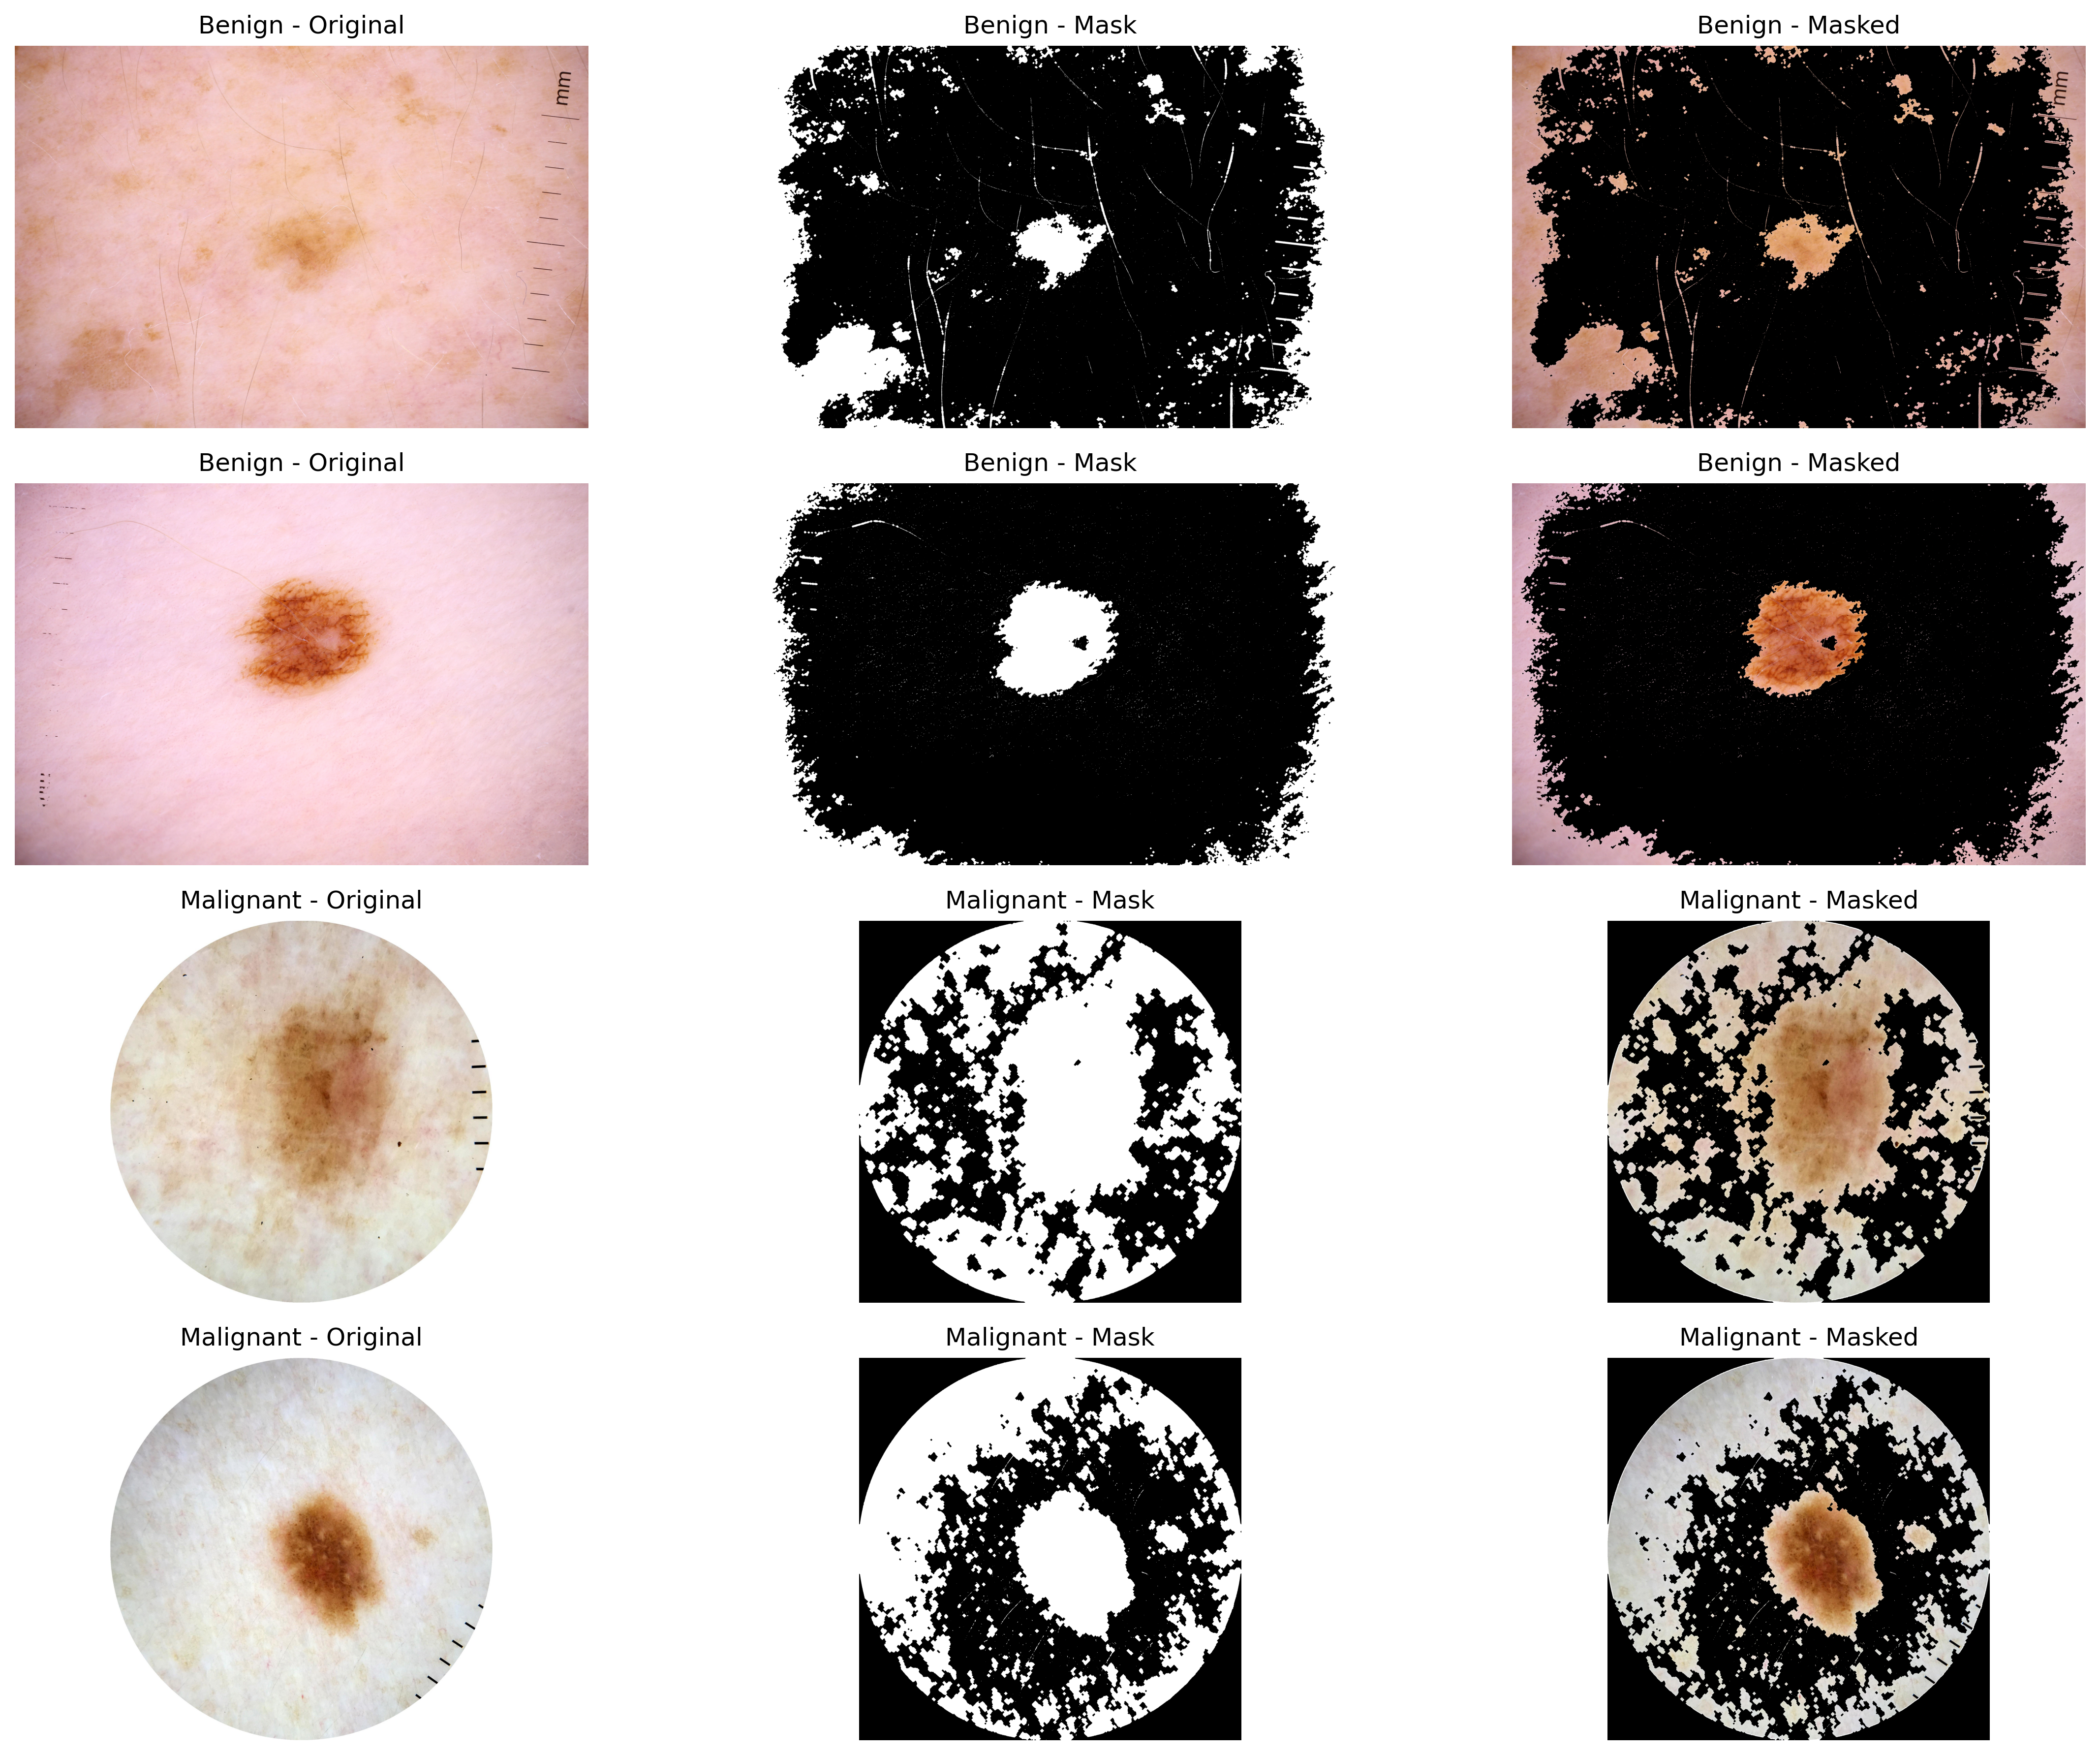
\includegraphics[width=\linewidth]{figures/dermoscopy_visualization.png}
\caption{Examples of benign and malignant images, their corresponding segmentation masks, and how segmentation-aided model inputs look after masking.}
\label{fig:segmentation-aided-inputs}
\end{figure}

\subsection{Segmentation masks in CIELAB}

To showcase an example of an image in the CIELAB color space and to demonstrate how masking appears in that space, we provide a visualization of a masked image:

\vspace{1em}
\begin{figure}[htbp]
\centering
\includegraphics[width=\linewidth]{figures/cielab_masked_image.jpeg}
\caption{Example of an image in CIELAB color space (visualized as RGB) after applying lesion segmentation.}
\label{fig:segmentation-cieelab}
\end{figure}


\subsection{Skin-former}

We refer to the technique of darkening images in the CIELAB color space as \textit{Skin-former}, an augmentation method aimed at reducing per-skin-type bias that a classification model might exhibit, especially since the distribution of skin color types is heavily imbalanced \cite{skin_color_debiasing}.

Such an uneven distribution presents a significant challenge, as our objective is to build a skin-type-agnostic classifier, mitigating any bias the model may have toward majority skin types. ISIC dataset mainly comprises of lighter skin color images.

To implement this, images are first converted from the RGB color space to the CIELAB color space. The \( L \) (lightness) and \( b \) (yellow-blue hue) components are then modified to simulate different Fitzpatrick Skin Types (FSTs). The transformation is based on a randomly selected target ITA value within the range of the desired FST. The new \( L \) and \( b \) components are calculated using Equations~\ref{eq:ita_diff}, \ref{eq:b_adjustment}, and \ref{eq:l_adjustment}.

\begin{myequation}[H]
\caption{ITA difference between original and target skin tone}
\label{eq:ita_diff}
\[
\Delta \text{ITA} = \text{ITA}_{\text{original}} - \text{ITA}_{\text{target}}
\]
\end{myequation}

\begin{myequation}[H]
\caption{Adjustment of the \textit{b} component in LAB space}
\label{eq:b_adjustment}
\[
b = b + (\Delta \text{ITA} \cdot 0.5)
\]
\end{myequation}

\begin{myequation}[H]
\caption{Adjustment of the \textit{L} component in LAB space}
\label{eq:l_adjustment}
\[
L = L - (\Delta \text{ITA} \cdot 0.12)
\]
\end{myequation}

Example of a side-by-side comparison of images before and after this augmentation can be seen in \ref{ap:skin_former}, here we present an example of this transformation.

\begin{figure}[ht]
    \centering
    \begin{subfigure}[b]{0.45\textwidth}
        \includegraphics[width=\linewidth]{figures/skin_former/ISIC_0081956.jpg}
        \caption{Original image}
        \label{fig:original_image}
    \end{subfigure}
    \hfill
    \begin{subfigure}[b]{0.45\textwidth}
        \includegraphics[width=\linewidth]{figures/skin_former/ISIC_0081956.jpg_shifted.png}
        \caption{Image after skin-former transformation. ITA was reduced by 46.28°, changing group to Brown.}
        \label{fig:augmented_image}
    \end{subfigure}
    \caption{Side-by-side comparison of image before and after skin-former augmentation.}
    \label{fig:sidebyside_skinformer}
\end{figure}

\section{Data samplers}

There are many different approaches to balancing datasets, such as undersampling the majority class, oversampling the minority class, using the \textit{Synthetic Minority Oversampling Technique (SMOTE)}, applying data augmentation strategies, or generating new samples with GANs (e.g., \textit{DermaGAN}).

In our work, we decided to utilize three types of data samplers:
\begin{itemize}
    \item Balanced batch sampler
    \item Imbalanced dataset sampler
    \item Undersampler
\end{itemize}

It is important to highlight the key distinction between the oversampler and the balanced batch sampler. While both can be used to generate a balanced benign–malignant dataset, the balanced batch sampler enforces equal class representation within each individual batch. In contrast, the oversampler does not guarantee balanced batches, meaning that a balance could, for instance, be achieved through a batch of only positives followed by a batch of only negatives.

\subsection{Balanced batch sampler vs undersampler}

Balanced batch sampler creates random duplicate records of malignant class samples. Given that we already apply augmentation techniques to mitigate the 49-to-1 class imbalance in favor of the benign class, it is evident that this approach could lead to overfitting.
In contrast, the undersampler suffers from information loss issues, primarily because it is not known a priori which benign images are hard to classify. Randomly dropping samples from the dataset can cause the model to perform worse, especially since a large portion of the dataset must be discarded to bring the number of benign samples closer to the number of malignant ones.

\vspace{1em}
\begin{figure}[htbp]
\centering
\includegraphics[width=\linewidth]{figures/over_vs_under_sampler.png}
\caption{Over- vs undersampler visualization.}
\label{fig:over_under_sampler}
\end{figure}

\subsection{Imbalanced dataset sampler}

To tackle the severe class imbalance present in the ISIC 2020 dataset, we experimented with a smarter oversampling strategy by integrating the \texttt{ImbalancedDatasetSampler}\footnote{\url{https://pypi.org/project/torchsampler/}} from the \texttt{torchsampler} library. This PyTorch sampler rebalances class distributions dynamically during training, without modifying or duplicating the dataset. Additionally, it automatically estimates sampling weights based on class frequencies. It avoids the need to create a new balanced dataset upfront, and when used with data augmentation, it can help mitigate overfitting by increasing sample variety.


\vspace{1em}
\begin{figure}[htbp]
\centering
\includegraphics[width=0.5\linewidth]{figures/imbalanced_dataset_sampler.png}
\caption{Imbalanced dataset sampler visualization.}
\label{fig:imbalanced_dataset_sampler}
\end{figure}

    \chapter{Modeling}
\label{ch:modeling}

In this section, we aim to discuss our choice of model architectures and how we utilized them in our solution. Beyond direct data manipulation, we also addressed the issue of severe class imbalance using advanced techniques designed to accommodate such imbalance and guide the model toward strong performance in detecting malignant lesions. We thoroughly examine the models, loss functions, class weighting strategies, model training, and the linear probing of selected models, as well as how we incorporated segmentation-aided training to support the fine-tuning process. Last section will discuss model fairness and how we design domain-aware training given the skin color groups/types.

\section{Model architectures}
\subsection{ConvNeXt}
ConvNeXt \cite{convnext2022} model architecture is a convolutional neural network architecture combining ideas of standard ConvNets with design principles inspired by transformer-based models like Vision Transformers (ViTs). It retains the efficiency and inductive biases of CNNs (like translation equivariance) while incorporating modern improvements such as large kernel sizes, layer normalization, and inverted bottlenecks. 
ConvNeXt models were supervisedly pretrained on the large-scale ImageNet-21K dataset and some were fine-tuned on ImageNet-1k. Best model achieved 87.8 acc@1 on ImageNet1k.

We thought of it as a good starting point due to several reasons: inductive biases, transfer learning, good performance on moderately sized datasets, and availability of papers using it for medical image processing( \cite{MedNeXt}, \cite{liu2023deep}).

\subsection{ConvNeXtV2}
The obvious next model to try was the ConvNeXtV2 architecture \cite{convnext_v2_2023}, a direct improvement over the original ConvNeXt. It leverages unsupervised pretraining via masked image modeling technique inspired by masked autoencoders in which the training objective is for the model to reconstruct the occluded parts of an image. Through this reconstruction-based pretraining, the model learns more effective feature representations. This was validated by experiments in which ConvNeXtV2 outperformed its predecessor on ImageNet-1K, achieving a then state-of-the-art accuracy of 88.9\%

What particularly drew our attention was the availability of fine-tuning recipes for a variety of tasks. These pretrained models performed well on downstream tasks such as classification, segmentation, and object detection, making ConvNeXtV2 a logical next choice for our problem.

\subsection{EfficientNetV2}

EfficientNetV2 \cite{efficientnetv2} is a family of CNN's that builds on the original EfficientNet architecture by introducing faster training, improved accuracy, and better scalability. It combines compound model scaling with progressive learning strategies and uses Fused-MBConv blocks in early layers for speed, while maintaining MBConv blocks in deeper layers for representational power. 
The model achieved 88.5\% accuracy on the ImageNet-1K dataset.

Our decision to explore EfficientNetV2 as one of the core architectures in our experiments was strongly motivated by its extensive adoption in the ISIC 2020 Challenge submissions. A large portion of the top-ranked solutions in that competition utilized one or more variants of EfficientNet, often as part of an ensemble, demonstrating the architecture’s practical effectiveness in skin lesion classification tasks. This widespread usage and good performance on this domain made it a logic choice to explore.


\subsection{DinoV2}

DINOv2 \cite{dinov2} is a self-supervised vision transformer model trained using the DINO (Self-Distillation with No Labels) framework. DINOv2 learns visual representations without labeled data by using a teacher-student training setup in which both networks process multiple views of the same image. The student network is trained to match the output of the teacher network, which is updated via exponential moving averages. This method encourages the model to learn semantically rich features.

DINOv2 is considered a foundation model in computer vision. As it was pretrained on a large-scale unlabeled dataset, the features obtained from the frozen DINOv2 can be used for linear probing, which means a classification head is attached to a model utilizing DINOv2 as the backbone and trained on top of its features to perform a downstream classification task. The idea is that DINOv2 features are semantically rich enough for the classification head to perform well.

It is also worth knowing that the authors in the ablation studies concluded that the model showcased no clear patterns indicating bias towards gender, skintones or age.

In the following figure from the original article, we can see how the first few PCA components of those features look like:

\begin{figure}[htbp]
\centering
\includegraphics[width=0.9\linewidth]{figures/dino_pca_comp_of_features.png}
\caption{Visualization of the first few PCA components of DINOv2 features (from the original DINOv2 paper)}
\label{fig:dino-pca}
\end{figure}


In our setting, we utilize DINOv2 in a linear probing setup. The backbone was frozen, and we trained only a lightweight classifier head on top of the extracted features. Since the majority of our models were prone to overfitting due to severe class imbalance, we believed this frozen-backbone setup could be particularly beneficial for achieving better generalization performance on our dataset.

\section{Loss functions and class weighting}

The ISIC 2020 challenge dataset has a 49-to-1 ratio of benign to malignant images. We tackled this issue using several dataset-level techniques (namely, oversampling, transformations of malignant images, etc.) as well as training-level sampling strategies (such as balanced batch samplers and oversamplers).

A common approach in computer vision tasks is to address this imbalance through custom loss functions that guide the model to focus either on harder-to-classify examples, on minority class samples, or on improving recall. In this section, we discuss how we used custom training objectives to increase the recall and F1 score for malignant class predictions.

\subsection{Cross-entropy}
As shown by \cite{dynamic_loss_balancing}, authors suggest that the interpretation of the standard cross-entropy loss is that it is a negative logarithm of the geometric mean of the correct class posterior:
\begin{myequation}
\caption{Cross-entropy as the negative log of the geometric mean of posteriors}
\label{eq:ce_geom}
\[
\text{CE} = -\frac{1}{N} \sum_{n=1}^{N} \ln P_n^{y_n} 
= -\frac{1}{N} \ln \prod_{n=1}^{N} P_n^{y_n} 
= -\ln \left( \prod_{n=1}^{N} P_n^{y_n} \right)^{\frac{1}{N}} 
= -\ln \overline{P}
\]
\end{myequation}


Cross entropy can also be view as summation of geometric means $P_c$ over all classes:
\begin{myequation}
\caption{Cross-entropy as a sum over class-wise log posteriors}
\label{eq:ce_weighted}
\[
\text{CE} = -\frac{1}{N} \sum_{c=1}^{C} \sum_{n: y_n = c} \ln P_n^c 
= -\sum_{c=1}^{C} \frac{1}{N} \ln \prod_{n: y_n = c} P_n^c 
= -\sum_{c=1}^{C} \frac{N_c}{N} \ln \left( \prod_{n: y_n = c} P_n^c \right)^{\frac{1}{N_c}} 
= -\sum_{c=1}^{C} \frac{N_c}{N} \ln \overline{P_c}
\]
\end{myequation}

Here, the set $\{n : y_n = c\}$ denotes all training examples belonging to class $c$, and $P_c = \left( \prod_{n: y_n = c} P_n^{y_n} \right)^{1/N_c}$ is the geometric mean of the predicted posteriors for class $c$.

As shown by equation~\eqref{eq:ce_weighted}, standard cross-entropy maximizes the arithmetic mean of the posterior geometric mean per class, with weights of each mean being occurrences of that class in the dataset. For any class imbalanced task, such partitioning is harmful as the bias for the majority class could prevail, which would result in the model always, or too often, predicting majority class/classes.


\subsection{Inverse Frequency Weighting (IFW)}

There are a couple of remedies for the imbalance problem shown in Equation~\eqref{eq:ce_weighted}.

Since cross-entropy can be expressed as
\begin{myequation}
\caption{Weighted cross-entropy expressed with per-class geometric means}
\label{eq:ce_weighted_2}
\[
\text{CE} = -\sum_{c=1}^{C} \frac{N_c}{N} \ln \overline{P_c}
\]
\end{myequation}
the first solution that comes to mind is to cancel out the weighting coefficients $\frac{N_c}{N}$. The technique known as inverse frequency weighting is a method of adjusting class contributions, where we multiply the biased weights in Equation~\eqref{eq:ce_weighted_2} by $\frac{N}{N_c} \cdot \alpha$, that is, by the inverse class frequency scaled by a factor $\alpha$, referred to as the correction coefficient, which is a training hyperparameter.

When using IFW cross entropy, equation~\eqref{eq:ce_weighted_2} deteriorates to : 
\begin{myequation}
\caption{IFW cross-entropy formula}
\label{eq:ce_ifw}
\[
\text{CE}_{\text{IFW}} = -\sum_{c=1}^{C} w_c \cdot \frac{N_c}{N} \ln P_c 
= -\sum_{c=1}^{C} \alpha \ln P
\]
\end{myequation}


\subsection{Recall-Based Cross-Entropy Loss}

As pointed out in \cite{dynamic_loss_balancing}, increasing the weights of minority classes can lead to a significant rise in false positives. The reason behind this is that standard cross-entropy is designed to consider only the posterior probability of the true class while ignoring the distribution over incorrect classes. This makes it suboptimal for our task, where we face a severe positive-to-negative class imbalance. For example, assigning 50 times more weight to malignant examples than benign ones can theoretically, and has experimentally, proven problematic, as it results in a surge of false positives. This often yields a recall of 1.00 but with extremely low precision.

To address this, \cite{dynamic_loss_balancing} proposes adapting loss weights based on the model’s recall performance. The idea is to begin training with inverse frequency-weighted cross-entropy and gradually reduce the weight assigned to the malignant class as its recall approaches 1.00. This allows the model to continue learning even after achieving perfect recall, ensuring gradient flow through the network, particularly to improve precision. In our case, the priority is to maximize recall for malignant examples, accepting the risk of lower precision, since class-imbalance techniques are intended to mitigate such trade-offs.
The exact equation follows:

\begin{myequation}
\caption{Recall-based class weighting formula}
\label{eq:recall_weight}
\[
w^{R}_{c,t} = \frac{N}{N_c} \left( 1 - R_{c,t} \right) + \epsilon
\]
\end{myequation}


Let us consider a simple example. Suppose we have a 50-to-1 negative-to-positive class ratio in a dataset with 10 malignant (positive) and 50 benign (negative) samples. If the model achieves a recall of 1.00 but produces 30 false positives, the resulting precision would be:
\[
\text{Precision} = \frac{10}{10 + 30} = 0.25 \quad (25\%)
\]
and the F1-score would be:
\[
\text{F1-score} = 2 \cdot \frac{\text{Precision} \cdot \text{Recall}}{\text{Precision} + \text{Recall}} = 2 \cdot \frac{0.25 \cdot 1.00}{0.25 + 1.00} = 0.40 \quad (40\%)
\]
However, one could argue that a 10\% false positive rate may be acceptable in our setting, given the importance of correctly identifying malignant cases.


\subsection{Online Hard Example Mining (OHEM)}

OHEM \cite{ohem} is a loss function technique originally designed for training deep neural networks on object detection tasks. It is based on the principle of distinguishing between easy-to-classify and hard-to-classify examples, with the goal of selecting and prioritizing the latter during training.

The objective of OHEM is to optimize model performance by focusing training on harder examples, rather than treating all examples equally. 

The training procedure involves calculating per-sample loss within each mini-batch, identifying the hardest examples (i.e., those with the highest loss values), and emphasizing them in subsequent training steps. These hard examples contribute more significantly to the gradient updates, as their higher loss values result in larger gradients, pushing the model to focus more on learning from them.

\subsection{Focal Loss}

Focal loss, proposed by \cite{focal_loss}, is a modified version of the standard cross-entropy loss designed to down-weight the contribution of well-classified examples and focus learning on hard, misclassified ones.

The authors argue that easily classified examples dominate the loss and gradients during training, which can stop learning, especially when a large class imbalance is present. While inverse-frequency weighting can address class imbalance, and methods like OHEM can be combined with it to focus on hard examples, such strategies may still lead to a bias toward misclassifying positive examples without explicitly addressing the rise in false positives. Focal loss addresses this by dynamically scaling the loss and reducing the contribution of easy negatives, thus acting as a balancing mechanism that emphasizes hard negatives during training.

The focal loss is defined as:
\begin{myequation}[H]
\caption{The focal loss formula}
\label{eq:focal_loss}
\[
\text{FL}(p_t) = - \alpha (1 - p_t)^{\gamma} \log(p_t)
\]
\end{myequation}

where:
\begin{itemize}
  \item \( p_t \) is the model’s estimated probability for the true class.
  \item \( \alpha \in [0, 1] \) is a balancing factor that compensates for class imbalance.
  \item \( \gamma \geq 0 \) is the focusing parameter that controls the rate at which easy examples are down-weighted.
\end{itemize}

The term \( (1 - p_t)^{\gamma} \) is the modulating factor that reduces the loss contribution of well-classified examples (i.e., those with high \( p_t \)).

Additionally, the authors experimented with introducing class priors into the model itself, ensuring that the estimated probability \( p \) for rare classes remains low at initialization. This helps shift early learning focus toward underrepresented (minority) classes.


\section{Probing vs fine-tuning}

In the model subsections, we stated that DINOv2 is a foundation model with large-scale pretraining that yields semantically rich image features suitable for linear probing. We implemented logic to freeze the model, attach a linear head on top of our module, which uses DINOv2 as a frozen backbone, and trained it; in other words, we linearly probed DINOv2 on the ISIC 2020 dataset.

Since DINOv2 was originally fine-tuned on 518$\times$518 resolution images, and given that we had access to an 8-GPU setup capable of processing large amounts of data at this resolution (especially when gradient flow is minimized during probing), we opted to use DINOv2-small with register hooks as our backbone extractor.

All other models in our pipeline were fine-tuned based on the available official fine-tuning recipes. Thanks to our support for multi-GPU distributed training, along with fine-grained control over numerous training hyperparameters, we were able to easily apply these official training procedures to fine-tune all the models we evaluated on the ISIC 2020 dataset.

In all cases, we used ImageNet-pretrained model checkpoints, removed the original classification head, and replaced it with a new binary classification head. Our implementation is modular and easily extendable. Adding new model architectures is straightforward, as demonstrated in the following model selection pseudocode:

\begin{algorithm}[H]
\caption{Backbone Selection in \texttt{MelanomaClassifier}}
\begin{algorithmic}[1]
\Function{MelanomaClassifier}{$model\_name, num\_classes, pretrained, in\_22k, freeze$}
    \If{$model\_name$ contains "convnext\_"}
        \State Load ConvNeXt backbone
        \State Replace head with \texttt{Linear(num\_features, num\_classes)}
    \ElsIf{$model\_name$ contains "efficientnet"}
        \State Load EfficientNetV2 with specified parameters
    \ElsIf{$model\_name$ contains "convnextv2"}
        \State Load ConvNeXtV2 with specified parameters
    \ElsIf{$model\_name$ contains "dinov2"}
        \State Load DINOv2 backbone, freeze it
        \State Append \texttt{Linear(num\_features, num\_classes)} to CLS output
    \Else
        \State Raise error: Unsupported model
    \EndIf
    \State \Return wrapped model
\EndFunction
\end{algorithmic}
\end{algorithm}


\section{Segmentation-assisted classification}

The authors \cite{skin_color_bias_ferit} explored the use of segmentation for skin lesion images. While they trained a dedicated segmentation module, we adopted a different approach. By employing hair mask removal and using Otsu's thresholding to segment pigmented regions of the skin, we generated masks that could be used for segmentation-aided classification.

The idea was to create binary masks and, during training, apply these masks to the input images so that only the lesion areas were preserved for the model to learn from and classify.

The biggest drawback of this approach was the reliability of the segmentation masks. Since they were generated using simple thresholding rather than learned segmentation, their quality was rather inconsistent. Another concern was the effectiveness of using pretrained models. Because these models were pretrained on datasets with very different input distributions, applying hard segmentation masks may result in a distribution shift that negatively affects transfer learning, potentially preventing the model from adapting during the training.


\section{Fairness in ML}

Fairness refers to acting justly, without favoritism or discrimination.  
Bias is defined as a systematic error in decision-making processes that results in unfair outcomes \cite{bias_vs_fairness}. Machine learning algorithms may exhibit several types of biases. The presence of any such bias undermines fairness. Bias can be introduced in various ways, including through the data, model design, user interactions, and more. In this work, we focus primarily on data-induced bias. Data bias arises when the dataset used to train machine learning models is unrepresentative or incomplete, leading to skewed selection or detection probabilities. As described in Chapter~\ref{ch:data_understanding}, the ISIC 2020 dataset exhibits a severe underrepresentation of darker skin types, as well as an imbalance between malignant and benign class examples \cite{fairness_review}. As discussed in Chapter~\ref{ch:business_understanding}, our objective is not only to achieve strong performance on the test dataset with respect to the target metric, but also to develop a model that actively mitigates bias.

Throughout this paper, we present the steps we have taken to reduce bias and increase fairness in our models. The machine learning community has long aimed to develop solutions that generalize well. It is widely accepted that truly generalizable models either contain minimal bias or are explicitly designed to mitigate it. For example, convolutional models carry an inductive bias toward spatial locality, which can aid generalization. Similarly, humans are biased to recognize objects by their shape, yet are still capable of generalization.

In our work, we aimed to train a model that is fair across skin tone groups by employing data augmentation techniques, preprocessing strategies, custom loss functions, intelligent sampling approaches, and skin tone-aware training procedures.

\subsection{Domain-aware training}

Domain-aware machine learning refers to the process of integrating knowledge or bias about the specific characteristics or distribution shifts of a given domain into the model training pipeline.

To successfully enable such training, the model's classification head, loss function, and evaluation procedure often need to be adjusted. However, if configured properly, the loss function can remain unchanged, as we will describe here, along with how to adapt the model for such training. The evaluation logic will be discussed separately in the following subsections.

In our case, the goal is not only to train a high-performing classifier according to an arbitrary target metric (e.g., recall), but also to ensure the model performs equitably well across different skin color groups. In other words, we aim to build a classifier that is domain-aware, with domains corresponding to skin color categories.

This implies two key assumptions: first, that we either know a priori or can infer the skin color group of each image; and second, that our baseline model does not perform equally across these groups. While the latter is difficult to validate given the imbalance in the skin color group distributions within our dataset, several studies have reported that classifiers are frequently biased toward certain groups \cite{skin_color_debiasing}, \cite{skin_color_bias_ferit}, \cite{assessing_bias_in_classifiers}, \cite{domain_aware_fairness}.

Our experiments did show that certain classifiers did have biases towards some skin colors, which will be explored in Section~\ref{ch:evaluation}.

\subsection{Fairness through awareness}
Authors \cite{fairness_through_awarness} propose an alternative to "fairness through blindness" by explicitly encoding domain information within the model, thereby directly mitigating domain bias. But what does domain information encoding mean?

In our case, the skin color groups (i.e., domains) are known a priori, as our dataset includes three ground-truth labels: target (whether the lesion is benign or malignant), group (the image's skin color group), and mask (the lesion segmentation mask). Given this, we can condition our model, specifically, the classification head, to be aware of the skin color group of each image. This enables the model to maintain orthogonal performance across domains by using multiple classification heads, each responsible for classifying targets within a specific domain.

Such a classifier is referred to as an ND-way classifier, where N is the number of classes and 
D is the number of domains. This leads to the first adaptation we apply to our classification head: instead of a standard 2-way classifier, it becomes an 8-way classifier, as we have 2 target classes and 4 skin color groups to evaluate against.

This structure unlocks an additional benefit: we can now apply inverse frequency weighting not just to individual classes, but to class-domain pairs, allowing for more granular handling of class imbalance across demographic subgroups.

\subsection{Prior shift inference}

Assume we have an ND-way classifier with a shared softmax layer. When interpreting model outputs as probabilities, a test-time inference strategy that suppresses class-domain correlation, which we refer to as domain-discriminative inference, can be formulated as:

\begin{myequation}[H]
\caption{Domain-discriminative inference formulation}
\label{eq:domain_disc_inf}
\[
\hat{y} = \arg\max_{y} \, P_{\text{test}}(y \mid x)
= \arg\max_{y} \sum_{d} P_{\text{test}}(y, d \mid x)
\]
\end{myequation}


In contrast to an ND-way classifier, a per-domain N-way classifier assumes domain-independent inference, which can be expressed as:

\begin{myequation}[H]
\caption{Domain-independent inference formulation}
\label{eq:domain_indep_inf}
\[
\hat{y} = \arg\max_{y} \sum_{d} s(y, d, x)
\]
\end{myequation}


The pseudocode for the latter is as follows:
\begin{algorithm}[H]
\caption{Domain-Discriminative Inference with Prior Shift}
\label{alg:prior_shift}
\begin{algorithmic}[1]
\Function{ComputePredictions}{$\texttt{outputs}, \texttt{num\_classes}, \texttt{num\_domains}$}
    \State Initialize $\texttt{prior\_weights} \gets$ predefined vector of length $N \cdot D$
    \State $\texttt{prior\_weights} \gets \texttt{prior\_weights} / 100$
    \State $\texttt{probs} \gets \texttt{Softmax(outputs)} \cdot \texttt{prior\_weights}$

    \For{$d = 1$ to $\texttt{num\_domains}$}
        \State Extract domain-specific class probs:
        \State \quad $\texttt{domain\_probs[d]} \gets \texttt{probs[:, d} \cdot \texttt{num\_classes} : (d{+}1) \cdot \texttt{num\_classes}]}$
    \EndFor

    \State $\texttt{summed\_probs} \gets \sum\limits_{d=1}^{D} \texttt{domain\_probs[d]}$ (element-wise sum over domains)
    \State $\texttt{predictions} \gets \arg\max\limits_{y} \texttt{summed\_probs}$ 
    \State \Return \texttt{predictions}
\EndFunction
\end{algorithmic}
\end{algorithm}





    \chapter{Evaluation}
\label{ch:evaluation}

Given the nature of this task, where we must aim for both fairness and performance, the role of model evaluation and selection is crucial. While this may seem straightforward, we will walk you through examples that highlight the challenges under these constraints.

Assume we have a test set \( y_t \), a subset of malignant images \( y_{t_m} \), and a subset of benign images \( y_{t_b} \). Let’s say we have a 50/50 ratio of malignant and benign examples, and that the dataset includes five skin tone groups, with each group comprising 10\% of the malignant and benign test images. Now assume we have a trained model \( m_1 \), which predicts all images in the test set as benign. Next, consider a second trained model \( m_2 \), which correctly identifies 40\% of malignant images as malignant. If benign examples represent true negatives, and malignant examples represent true positives, we can say the following:

\begin{itemize}

\item Model \( m_1 \) has a recall of 0\%. It performs equally across all five skin tone groups, not because it performs well, but because it fails consistently. This model is clearly unusable in practice, but from a fairness standpoint, it is unbiased. It shows no preferential treatment toward any group, as the recall is 0\% for all.

\item Model \( m_2 \) has a recall of 80\%, precision of 90\%, and an F1 score of 85\%. At first glance, we would consider this a well-performing model. However, consider the fairness implications: since each group has 10\% of the malignant images, the model must fail evenly across groups to be considered fair. If, for example, the model misses all malignant images belonging to group 1, and none from the other groups, the performance difference in recall across groups would be 100\%. That’s an extreme disparity, and even though the overall performance is high, such bias would be unacceptable.

\end{itemize}

We haven’t yet formally introduced fairness metrics, but this example gives an intuitive hint: our goal is to increase recall for malignant images across all groups. A fair model cannot have a 100\% difference in its target metric (such as recall) across demographic groups, regardless of how well it performs overall. In the following sections, we will explain the metrics used for model evaluation, how we tested for model bias, present our experiments and results, and describe how we ultimately selected our final model.

\section{Metrics}

Benign images are true negatives, malignant images are true positives. Mistaking benign image for benign is false negative, mistaking benign image for malignant is false positives.

\subsection{Standard computer vision metrics}

\begin{myequation}[H]
\caption{Accuracy as the ratio of correctly predicted samples to all samples}
\label{eq:accuracy}
\[
\text{Accuracy} = \frac{TP + TN}{TP + TN + FP + FN}
\]
\end{myequation}


Recall, or true positives rate, is defined as the number of positive samples correctly classified by the model, divided by the total number of actual positive samples:

\begin{myequation}[H]
\caption{Recall as the ratio of true positives to all actual positives}
\label{eq:recall}
\[
\text{Recall} = \frac{TP}{TP + FN}
\]
\end{myequation}

Precision is the number of correctly identified positive samples, divided by the total number of samples predicted as positive:

\begin{myequation}[H]
\caption{Precision as the ratio of true positives to all predicted positives}
\label{eq:precision}
\[
\text{Precision} = \frac{TP}{TP + FP}
\]
\end{myequation}


The F1 score is the harmonic mean of precision and recall:

\begin{myequation}[H]
\caption{F1 score as the harmonic mean of precision and recall}
\label{eq:f1}
\[
\text{F1 Score} = 2 \cdot \frac{\text{Precision} \cdot \text{Recall}}{\text{Precision} + \text{Recall}}
\]
\end{myequation}


The false positive rate (FPR) indicates the probability of predicting a positive class when the actual class is negative.

\begin{myequation}[h!]
\caption{False positive rate (FPR)}
\label{eq:fpr}
\[
\text{FPR} = \frac{FP}{FP + TN}
\]
\end{myequation}

A false positive error, also known as a Type I error in statistics (denoted by $\alpha$), occurs when a model incorrectly rejects a true null hypothesis, in other words, it predicts a positive class when the true class is negative.

The false negative rate (FNR) is the proportion of actual positives that are incorrectly classified as negative. It is defined as one minus recall:

\begin{myequation}[h!]
\caption{False negative rate (FNR)}
\label{eq:fnr}
\[
\text{FNR} = \frac{FN}{FN + TP} = 1 - \text{Recall}
\]
\end{myequation}

A false negative error, or Type II error in statistics (denoted by $\beta$), occurs when a model fails to detect the positive class.

The true negative rate (TNR), also known as specificity, measures the proportion of actual negatives that are correctly classified:

\begin{myequation}[h!]
\caption{True negative rate (Specificity)}
\label{eq:tnr}
\[
\text{TNR} = \frac{TN}{TN + FP}
\]
\end{myequation}

Balanced accuracy is a commonly used metric in binary classification that is especially useful for imbalanced datasets. It is the average of recall (sensitivity) and specificity:

\begin{myequation}[h!]
\caption{Balanced accuracy}
\label{eq:balanced_accuracy}
\[
\text{Balanced Accuracy} = \frac{\text{Recall} + \text{Specificity}}{2}
\]
\end{myequation}


\subsection{Fairness metrics}

Selection rate is a metric that indicates the proportion of samples predicted as positive out of all samples. In the context of melanoma detection, it reflects how frequently the model predicts that an image is malignant.

\begin{myequation}
\caption{Selection rate (positive prediction rate)}
\label{eq:selection_rate}
\[
\text{Selection Rate} = \frac{TP + FP}{TP + FP + TN + FN} 
\]
\end{myequation}

We use this metric as a fairness indicator that reflects how often the model selects images as malignant. Since malignant cases are underrepresented in our dataset, we aim for the model to identify more of them, even at the cost of increased false positives, because false negatives are more critical in a real world scenario. Furthermore, we examine this metric across different skin tone groups, where selection rate reveals whether certain groups are more likely to be predicted as malignant, indicating bias.

Demographic parity difference (DPD) is a disparity m that measures whether the probability of a sample being predicted as positive (malignant) is independent of the group it belongs to (skin color group). 
Demographic parity is achieved when the selection rate is equal across all groups. A DPD of 0 indicates perfect parity, while a DPD of 100pp indicates maximum disparity between groups.


\begin{myequation}[H]
\caption{Demographic parity difference}
\label{eq:dpd}
\[
\text{DPD} = \max_{g_1, g_2} \left| \text{SelectionRate}_{g_1} - \text{SelectionRate}_{g_2} \right|
\]
\end{myequation}

This metric clearly highlights the issue described in Section~\ref{ch:evaluation}, where two models are compared. In the second example, a DPD of 100 would indicate that one skin tone group was completely neglected, suggesting the model is highly biased.


Equalized odds was proposed to address the limitations of the DPD metric. While DPD is a good indicator of overall selection rate disparities across different skin tone groups, it may fail to detect cases where a model has similar selection rates but significantly different error rates between groups. For instance, a model could show equal selection rates while having a much higher false positive rate for a specific group, thus revealing bias undetected by DPD. Equalized Odds considers both the true positive rate (TPR) and the false positive rate (FPR) across groups. This parity constraint is satisfied when both of these rates are equal for all groups:

\begin{myequation}[H]
\caption{Equalized odds}
\label{eq:equalized_odds}
\[
\text{TPR}_{g_1} = \text{TPR}_{g_2} \quad \text{and} \quad \text{FPR}_{g_1} = \text{FPR}_{g_2}
\]
\end{myequation}

Equal opportunity is a relaxed version of equalized odds. Instead of requiring both TPR and FPR to be equal across groups, it only requires the true positive rates to be equal. This means the metric only considers the model’s ability to correctly detect the positive class (malignant cases in our case), and allows for variation in FPR between groups.
This assumption is justifiable in our use case: we aim for fair performance primarily across malignant examples. The rationale is simple: if we must trade off some false positives in benign cases to improve sensitivity  for malignant cases, that is a  acceptable and fairness-aligned decision.

\begin{myequation}
\caption{Equal opportunity}
\label{eq:equalized_opportunity}
\[
\text{TPR}_{g_1} = \text{TPR}_{g_2}
\]
\end{myequation}


\section{Results}
\label{sec:results}

We trained our models on an 8-GPU cluster using a cosine scheduler \cite{cosine_scheduler}, the AdamW optimizer \cite{adamw}, full precision training, and input images with a resolution of 224×224. We artificially augmented our malignant image subset using horizontal flips, vertical flips, random rotations of less than 15 degrees, and slight translation. We also experimented with ColorJitter, but decided not to include it as a standard augmentation, as we were concerned it might distort the specific pigmentation patterns of malignant lesions. We experimented with different data samplers, models, loss functions, color spaces (RGB vs. CIELAB), learning rates, training hyperparameters, domain-aware training strategies, skin masking techniques, skin color transformations, and strategies such as linear probing versus full fine-tuning. We present our results in the form of tables, often comparing similar experiments and identifying the best-performing models based on a combination of F1 score, false negative rate, and fairness metrics such as Demographic Parity Difference (DPD), Equalized Odds, and Equal Opportunity. Some training runs are not shown in the tables but are discussed in the appendix \ref{ap:model_results}.

\subsection{Baseline model}

The baseline model is a ConvNeXt-Tiny architecture, which has 28 million parameters and 4.5 GFLOPs. We use the variant pretrained on ImageNet-22k and fine-tuned on ImageNet-1k with an input resolution of 224×224. We applied augmentations to the malignant subclass, used a learning rate of 5e-5, and set the weight decay to 5e-3. The model was trained for 10 epochs using RGB images and inverse frequency weighting with the standard cross-entropy loss.

\begin{table}[h!]
\centering
\caption{ Results of our baseline model - ConvNeXt Tiny model with input resolution 224x224, using inverse-frequency weighting and RGB colorspace.}
\resizebox{\textwidth}{!}{%
\begin{tabular}{|c|c|c|c|c|c|c|c|c|}
\toprule
 epoch &  train loss &  train acc &  test loss &  test acc &  test malignant recall &  test malignant precision &  test malignant f1 &  test malignant recall diff \\
\midrule
     0 &    2.231950 &         0.382633 &   0.582571 &  77.293508 &               0.839416 &                  0.072647 &           0.133721 &            0.072008 \\
     1 &    1.319754 &         0.756773 &   0.537405 &  77.918318 &               0.868613 &                  0.076774 &           0.141079 &            0.206897 \\
     2 &    0.909625 &         0.841313 &   0.418328 &  82.627248 &               0.839416 &                  0.093268 &           0.167883 &            0.234280 \\
     3 &    0.523071 &         0.909045 &   0.244960 &  90.231637 &               0.671533 &                  0.133721 &           0.223030 &            0.236573 \\
     4 &    0.299384 &         0.949326 &   0.169093 &  95.062481 &               0.547445 &                  0.222552 &           0.316456 &            0.475659 \\
     5 &    0.220884 &         0.965776 &   0.387288 &  87.336178 &               0.781022 &                  0.117841 &           0.204785 &            0.175456 \\
     6 &    0.122728 &         0.979286 &   0.117246 &  96.860713 &               0.452555 &                  0.321244 &           0.375758 &            0.419878 \\
     7 &    0.040332 &         0.992582 &   0.110418 &  97.485523 &               0.386861 &                  0.395522 &           0.391144 &            0.454361 \\
     8 &    0.018326 &         0.997133 &   0.115302 &  97.759829 &               0.372263 &                  0.455357 &           0.409639 &            0.471602 \\
     9 &    0.012803 &         0.998172 &   0.116700 &  97.744590 &               0.364964 &                  0.450450 &           0.403226 &            0.482097 \\
\bottomrule
\end{tabular}
} % end of resizebox
\end{table}

\vspace{1em}
\begin{figure}[H]
\centering
\includegraphics[width=\linewidth]{figures/results/baseline_experiment_loss_per_epoch.png}
\caption{Training and test loss per epoch for the baseline model.}
\label{fig:baseline-loss}
\end{figure}

\vspace{1em}
\begin{figure}[H]
\centering
\includegraphics[width=\linewidth]{figures/results/baseline_experiment_metricsper_epoch.png}
\caption{F1 score, recall, and precision of the malignant class across epochs in the baseline model.}
\label{fig:baseline-metrics}
\end{figure}


What we observe in this table and on the graphs is that the model converges on both the training and test sets. Convergence on the training set is evident from the gradual decrease in loss, which approaches zero, and the training accuracy reaching nearly 100\%. This is a common effect we noticed where the model easily learns to find the decision boundary between the smaller number of malignant examples and the more abundant benign ones in the training set, yet this does not translate well to test performance. We also concluded that the test recall from the best epoch, based on the highest F1 score in the 9\textsuperscript{th} epoch (37.22\%), was too low. Our goal then became to improve recall for the malignant class while maintaining the F1 score as much as possible.

\subsection{Baseline vs recall cross entropy}
We immediately started an ablation regarding the performance of recall based loss compared to weighted croos entropy loss. Then we did an ablation of parameter tuning experiments, and here we report the best example. 

\begin{table}[H]
\centering

\caption{Comparison of three configurations showing test accuracy, recall, F1, DPD, and group-wise recall for the malignant class.}
\resizebox{\textwidth}{!}{%
\begin{tabular}{|l|c|c|c|c|c|c|c|c|}
\toprule
\textbf{Experiment} & \textbf{Test Acc} & \textbf{Test Recall} & \textbf{Test F1} & \textbf{Test DPD} & \textbf{Group 0 Recall} & \textbf{Group 1 Recall} & \textbf{Group 3 Recall} & \textbf{Group 4 Recall} \\
\midrule
Baseline CE + IFW & 97.8\% & 37.2\% & 41.0\% & 4.39\% & 76.5\% & 29.3\% & 30.4\% & 43.8\% \\
Recall recall\_based CE & 96.2\% & 50.4\% & 35.8\% & 7.70\% & 76.5\% & 44.8\% & 45.7\% & 56.3\% \\
\bottomrule
\end{tabular}
} % end of resizebox
\label{tab:baseline-vs-variants}
\end{table}

These results show that recall indeed increased, but at the cost of precision, resulting in lower F1 scores. We attempted to scale up the model, but no improvements were observed. Therefore, we decided to take a different approach: we switched to the CIELAB color space. All experiments from this point onward will use CIELAB images.

\subsection{CIELAB colorspace results}

All of the reported results use the same model: ConvNeXt Tiny, adamw optimizer, cosine scheduler, input resolution of 224x224, and CIELAB normalization based on mean and std of ISIC CHallenge datset in CIELAB colorspace.

\begin{table}[H]
\centering
\caption{Comparison of selected ConvNeXt Tiny experiments on CIELAB images.}
\resizebox{\textwidth}{!}{%
\begin{tabular}{|l|c|c|c|c|c|c|c|c|}
\toprule
\textbf{Experiment} & \textbf{Test Acc} & \textbf{Test Recall} & \textbf{Test F1} & \textbf{Test DPD} & \textbf{Group 0 Recall} & \textbf{Group 1 Recall} & \textbf{Group 3 Recall} & \textbf{Group 4 Recall} \\
\midrule
Recall based CE & 93.6\% & 56.2\% & 27.0\% & 12.5\% & 70.6\% & 43.1\% & 63.0\% & 68.8\% \\
OHEM + ifw & 96.6\% & 32.8\% & 28.6\% & 4.91\% & 64.7\% & 22.4\% & 30.4\% & 43.8\% \\
Finetune of 1 for 10 epochs & 91.9\% & 54.7\% & 22.1\% & 18.2\% & 64.7\% & 46.6\% & 58.7\% & 62.5\% \\
Recall based CE 50 epochs & 95.2\% & 43.8\% & 27.4\% & 19.6\% & 82.4\% & 32.8\% & 45.7\% & 37.5\% \\
Oversampler + re & 94.5\% & 49.6\% & 27.5\% & 9.49\% & 82.4\% & 37.9\% & 54.4\% & 43.8\% \\
Focal loss & 97.0\% & 29.9\% & 29.2\% & 4.57\% & 70.6\% & 20.7\% & 30.4\% & 18.8\% \\
\bottomrule
\end{tabular}
} % end of resizebox
\label{tab:selected-experiments}
\end{table}

These experiments showed a slight increase in recall compared to the RGB color space; an improvement of 5.8\%, from 50.4\% to 56.2\%.  
The F1 score consistently remained below the 30\% mark, and we generally observed that higher overall recall was associated with lower DPD values.  
From the table, we can also see that we have not yet reached satisfactory recall levels, as Groups 1 and 3 still show notably lower recall compared to others.
We still haven't taken a look at the fairness of our models, except for DPD, and we will few sections below. We are still aiming to increase the recall.
In the ablation \ref{ap:model_results}, table \ref{tab:oversampler_abl}, we did ablation study concerning which loss to use with oversampler.

\subsection{EfficientNetV2 experiments}
We did and extensive EfficientNetV2 experiment ablation, here we are reporting two of our best runs.

\begin{table}[h!]
\centering
\caption{Performance comparison between EfficientNet-M and Efficient-L models.}
\resizebox{\textwidth}{!}{%
\begin{tabular}{|l|c|c|c|c|c|c|c|c|}
\toprule
\textbf{Experiment} & \textbf{Test Acc} & \textbf{Test Recall} & \textbf{Test F1} & \textbf{Test DPD} & \textbf{Group 0 Recall} & \textbf{Group 1 Recall} & \textbf{Group 3 Recall} & \textbf{Group 4 Recall} \\
\midrule
EfficientNetV2 M + recall based CE + IFW & 92.4\% & 56.9\% & 23.8\% & 14.0\% & 82.4\% & 44.8\% & 58.7\% & 68.8\% \\
EfficientNetV2 L + recall based CE + IFW & 94.0\% & 50.4\% & 26.0\% & 9.65\% & 94.1\% & 39.7\% & 43.5\% & 62.5\% \\
\bottomrule
\end{tabular}
} % end of resizebox
\label{tab:efficient-models}
\end{table}

These models showed little progress in teh direction we wanted: to increase recall and F1 score. EfficientNetV2 M  got the highest recall so far, EfficientNetV2 L struggled with overfitting the train dataset.
We decided to apply heavier transformations: segmentation-aided classification and skin-former based modelling.

\subsection{Segmentation-aided classification and skin-former results}

We aimed to evaluate the performance of the ConvNeXt-Tiny model, which is capable of handling irregular image inputs, on two types of data: segmented images, where only the lesions were visible to the model, and color-transformed images, referred to as the skin-former approach.

\begin{table}[H]
\centering
\caption{Performance of ConvNeXt-Tiny on 224x224 CIELAB images with skin color transformer augmentation and masked skin augmentation.}
\resizebox{\textwidth}{!}{%
\begin{tabular}{|l|c|c|c|c|c|c|c|c|}
\toprule
\textbf{Experiment} & \textbf{Test Acc} & \textbf{Test Recall} & \textbf{Test F1} & \textbf{Test DPD} & \textbf{Group 0 Recall} & \textbf{Group 1 Recall} & \textbf{Group 3 Recall} & \textbf{Group 4 Recall} \\
\midrule
Skin former + Recall based CE & 90.3\% & 66.4\% & 22.3\% & 17.6\% & 88.2\% & 51.7\% & 69.6\% & 87.5\% \\
Skin former + OHEM + IFW & 96.0\% & 31.4\% & 24.8\% & 5.09\% & 58.8\% & 27.6\% & 28.3\% & 25.0\% \\
Masked skin + Recall based CE & 96.0\% & 37.2\% & 25.7\% & 10.1\% & 82.4\% & 24.1\% & 39.1 \% & 31.3\% \\
\bottomrule
\end{tabular}
} % end of resizebox
\label{tab:transformer-results}
\end{table}

The masked skin transformation resulted in a performance decrease compared to previous results. We believe the explanation lies in the fact that we were using pretrained weights on ImageNet, and this data distribution shift proved insurmountable for our model to overcome. 
Additionally, this transformation often produced a higher number of false positives and led to unstable training when not initialized with pretrained weights, as the models easily overfitted the training dataset. We therefore decided not to experiment further with this transformation.
As a result, we turned to the skin-former transformation for ablation studies, aiming to improve these results. It proved easier to train with, yielded a 9.5\% higher recall than EfficientNetV2-M, and produced fewer false positives across demographic groups.
A natural next step was to apply domain-aware training. The following section presents the best of those runs.


\subsection{Domain-aware training}
Here, we report three of our best runs using the skin-former augmentation and domain-aware training setup. We experimented with both domain-independent and domain-discriminative training strategies, and present the results below.


\begin{table}[H]
\centering
\caption{Performance of domain-discriminatively and domain-independently trained ConvNeXt-Tiny models using 224×224 CIELAB images with optional skin-former augmentation.}
\label{tab:domain-transformers}
\resizebox{\textwidth}{!}{%
\begin{tabular}{|l|c|c|c|c|c|c|c|c|}
\toprule
\textbf{Experiment} & \textbf{Test Acc} & \textbf{Test Recall} & \textbf{Test F1} & \textbf{Test DPD} & \textbf{Group 0 Recall} & \textbf{Group 1 Recall} & \textbf{Group 3 Recall} & \textbf{Group 4 Recall} \\
\midrule
Domain discriminative + CE + IFW & 89\% & 72.3\% & 21.5\% & 18.9\% & 88.2\% & 62.1\% & 73.9\% & 87.5\% \\
Domain independent + CE + IFW & 97\% & 19.7\% & 23.5\% & 2.10\% & 29.4\% & 17.2\% & 19.6\% & 18.8\% \\
Domain discriminative + skin former + CE + IFW & 85\% & 23.8\% & 17.4\% & 25.4\% & 82.4\% & 62.1\% & 82.6\% & 87.5\% \\
\bottomrule
\end{tabular}
} % end of resizebox

\end{table}

Domain-independent training underperformed on the test set. It consistently predicted the majority of images as benign, resulting in regularly low recall. Forcing the model to learn the decision boundary between classes only increased the false positive rate and reduced precision. Therefore, we decided not to continue with this training procedure.
On the other hand, the domain-discriminative training procedure yielded the highest recall scores across all runs. The best run increased recall by 8.1\%, reaching a strong overall recall of 74.5\%. When analyzing group-wise recall, the lowest was recorded in Group 1 with 62.1\%, while all other groups achieved well over 80\% recall.

We were willing to sacrifice some precision, which came at the cost of a drop in F1 score, from the baseline of 40\% down to as low as 17.4\%. Given the 49-to-1 imbalance ratio in our dataset, we considered this trade-off acceptable, as we could afford more false positives and a higher false positive rate.

\subsection{Fairness analysis}
We conducted an extensive fairness analysis of most of our models; here, we present a shortened version of the results table. The full table is provided in Appendix~\ref{ap:model_results}.

Our primary condition was that the model must maintain a low false positive rate: our priority was recall, and we could not afford to lower recall in favor of a higher F1 score. This was a general tendency across all models: they would either predict more malignant cases, boosting recall but reducing F1 score due to more false positives, or increase F1 during training at the cost of recall by maintaining a low false positive rate. Some of our experiments, which are discussed in Appendix~\ref{ap:model_results}, either overfitted the training data or, in the case of linear probing with DINOv2, underfitted, resulting in an overwhelming number of false positives, with 100\% recall but precision of only a few percentage points.

It was difficult to establish rigid criteria, but we ultimately used the following thresholds: 
\begin{itemize}
    \item False negative rate over 50\% was considered unacceptable and such models were excluded.
    \item False positive rate over 50\% was another exclusion criterion, which only applied to linear probing experiments (see Appendix~\ref{ap:model_results}).
    \item Recall lower than 50\% was considered insufficient.
    \item Lastly, an F1 score below 20\% was deemed inadequate for inclusion.
\end{itemize}

It is worth noting that only one model per architecture and training configuration was retained. Among models that met these thresholds, the EfficientNetV2-M model achieved 56\% recall and a 24\% F1 score, compared to the best EfficientNetV2-L model, which had a 2\% higher F1 but 6\% lower recall. In this case, we chose the smaller M variant, as higher recall and fewer parameters were prioritized over a marginally better F1 score.
The table summarizing the best-performing models and metrics across the entire validation dataset is presented below:


\begin{table}[H]
\centering
\caption{Comparison of selected experiments across fairness and classification metrics.}
\resizebox{\textwidth}{!}{%
\begin{tabular}{|l|c|c|c|c|c|c|c|c|}
\toprule
\textbf{Experiment} & \textbf{Balanced Acc.} & \textbf{DPD} & \textbf{Eq. Opp.} & \textbf{F1} & \textbf{FNR} & \textbf{FPR} & \textbf{Recall} & \textbf{Selection Rate} \\
\midrule
ConvNeXt-tiny + RGB + recall CE & 73.78\% & 7.70\% & 31.64\% & 35.75\% & 49.64\% & 2.80\% & 50.37\% & 3.79\% \\
ConvNeXt-tiny + CIELAB + recall CE & 75.32\% & 12.50\% & 27.48\% & 26.97\% & 43.80\% & 5.56\% & 56.20\% & 6.61\% \\
ConvNeXt-tiny + skin-former & 78.62\% & 17.55\% & 36.51\% & 22.25\% & 33.58\% & 9.18\% & 66.42\% & 10.38\% \\
ConvNeXt-tiny + domain discriminative train & 80.81\% & 18.86\% & 26.17\% & 21.52\% & 27.74\% & 10.65\% & 72.26\% & 11.93\% \\
EfficientNet-M + recall CE + IFW & 75.04\% & 13.95\% & 37.53\% & 23.82\% & 43.07\% & 6.85\% & 56.93\% & 7.89\% \\
\bottomrule
\end{tabular}
} % end of resizebox
\label{tab:fairness-metrics}
\end{table}

We emphasize that the results discussed here are based on validation over the entire dataset. These metrics offer a broader view of our model performances, but they do not allow for a fine-grained assessment of bias at the individual skin color group level. First, let us examine some general conclusions drawn from this table.

The Demographic Parity Difference (DPD) reaches a maximum of around 19\%, signaling the model with the largest performance disparity across groups. The lowest DPD observed was 8\%. When comparing this with recall, and acknowledging their potential mutual exclusiveness, we see that the model with the highest recall also exhibited the highest DPD, while the model with the lowest recall had the lowest DPD. This could suggest that the best-performing model in terms of recall learned patterns specific to one skin color group more effectively than others. However, this observation alone does not provide a definitive answer as to which model is preferable.

The Equal opportunity metric generally indicated similar performance across models. We stress that this metric was calculated using the validation dataset only and represents the probability of a positive case being correctly identified, conditional on the individual's group. Again, the model with the highest recall showed the lowest equalized opportunity score. However, this metric ranged fairly consistently between 26\% and 37\% across all models.

The model with the highest recall also produced the most predictions, which led to more false positives than other models. This is reflected in its highest false positive rate and highest selection rate. At the same time, it achieved the lowest false negative rate among all models. Naturally, a higher selection rate and false positive rate result in lower precision; thus, it is not surprising that this model also had the lowest F1 score, at 21.52\%.

\subsubsection{Group-level metrics}
Let us further analyze these models of ours. We are now digging deeper: at the per-group prediction level.

\begin{table}[htpb]
\centering
\caption{Per-group performance metrics: ConvNeXt-tiny + RGB + recall CE}
\label{tab:rgb-recallce} 
\begin{tabular}{cccccccc}
\toprule
\textbf{Group} & \textbf{F1} & \textbf{Recall} & \textbf{Accuracy} & \textbf{\begin{tabular}[c]{@{}c@{}}Selection\\ Rate\end{tabular}} & \textbf{\begin{tabular}[c]{@{}c@{}}Balanced \\ Accuracy\end{tabular}} & \textbf{FPR} & \textbf{FNR} \\ \midrule
0              & 60\%        & 76\%            & 94\%              & 9\%                                                               & 86\%                                                                  & 5\%          & 24\%         \\
1              & 31\%        & 45\%            & 97\%              & 3\%                                                               & 71\%                                                                  & 2\%          & 55\%         \\
2              & 31\%        & 46\%            & 94\%              & 5\%                                                               & 71\%                                                                  & 4\%          & 54\%         \\
3              & 46\%        & 56\%            & 91\%              & 10\%                                                              & 75\%                                                                  & 7\%          & 44\%         \\ \bottomrule
\end{tabular}
\end{table}

\begin{table}[htpb]
\centering
\caption{Per-group performance metrics: ConvNeXt-tiny + CIELAB + recall CE}
\label{tab:ciellab-recallce}
\begin{tabular}{cccccccc}
\toprule
\textbf{Group} &
  \textbf{F1} &
  \textbf{Recall} &
  \textbf{Accuracy} &
  \textbf{\begin{tabular}[c]{@{}c@{}}Selection\\ Rate\end{tabular}} &
  \textbf{\begin{tabular}[c]{@{}c@{}}Balanced \\ Accuracy\end{tabular}} &
  \textbf{FPR} &
  \textbf{FNR} \\ \midrule
0 & 62\% & 71\% & 95\% & 8\%  & 83\% & 4\%  & 29\% \\
1 & 21\% & 43\% & 96\% & 4\%  & 70\% & 3\%  & 57\% \\
2 & 24\% & 63\% & 88\% & 12\% & 76\% & 11\% & 37\% \\
3 & 42\% & 69\% & 86\% & 16\% & 78\% & 12\% & 31\% \\ \bottomrule
\end{tabular}
\end{table}

\begin{table}[htpb]
\centering
\caption{Per-group performance metrics: ConvNeXt-tiny + skin-former}
\label{tab:skin-former}
\begin{tabular}{cccccccc}
\toprule
\textbf{Group} &
  \textbf{F1} &
  \textbf{Recall} &
  \textbf{Accuracy} &
  \textbf{\begin{tabular}[c]{@{}c@{}}Selection\\ Rate\end{tabular}} &
  \textbf{\begin{tabular}[c]{@{}c@{}}Balanced \\ Accuracy\end{tabular}} &
  \textbf{FPR} &
  \textbf{FNR} \\ \midrule
0 & 59\% & 88\% & 93\% & 12\% & 91\% & 7\%  & 12\% \\
1 & 16\% & 52\% & 93\% & 7\%  & 73\% & 6\%  & 48\% \\
2 & 19\% & 70\% & 83\% & 18\% & 77\% & 16\% & 30\% \\
3 & 39\% & 88\% & 81\% & 24\% & 84\% & 20\% & 13\% \\ \bottomrule
\end{tabular}
\end{table}

\begin{table}[htpb]
\centering
\caption{Per-group performance metrics: ConvNeXt-tiny + domain discriminative}
\label{tab:domain-discriminative}
\begin{tabular}{cccccccc}
\toprule
\textbf{Group} &
  \textbf{F1} &
  \textbf{Recall} &
  \textbf{Accuracy} &
  \textbf{\begin{tabular}[c]{@{}c@{}}Selection\\ Rate\end{tabular}} &
  \textbf{\begin{tabular}[c]{@{}c@{}}Balanced \\ Accuracy\end{tabular}} &
  \textbf{FPR} &
  \textbf{FNR} \\ \midrule
0 & 56\% & 88\% & 92\% & 13\% & 90\% & 8\%  & 12\% \\
1 & 17\% & 62\% & 92\% & 8\%  & 77\% & 8\%  & 38\% \\
2 & 19\% & 74\% & 82\% & 20\% & 78\% & 18\% & 26\% \\
3 & 36\% & 88\% & 78\% & 27\% & 83\% & 22\% & 13\% \\ \bottomrule
\end{tabular}
\end{table}

\begin{table}[htpb]
\centering
\caption{Per-group performance metrics: EfficientNet-M}
\label{tab:efficientnet-m}
\begin{tabular}{cccccccc}
\toprule
\textbf{Group} &
  \textbf{F1} &
  \textbf{Recall} &
  \textbf{Accuracy} &
  \textbf{\begin{tabular}[c]{@{}c@{}}Selection\\ Rate\end{tabular}} &
  \textbf{\begin{tabular}[c]{@{}c@{}}Balanced \\ Accuracy\end{tabular}} &
  \textbf{FPR} &
  \textbf{FNR} \\ \midrule
0 & 55\% & 82\% & 92\% & 12\% & 87\% & 7\%  & 18\% \\
1 & 18\% & 45\% & 95\% & 5\%  & 70\% & 5\%  & 55\% \\
2 & 21\% & 59\% & 87\% & 13\% & 73\% & 12\% & 41\% \\
3 & 37\% & 69\% & 84\% & 19\% & 77\% & 15\% & 31\% \\ \bottomrule
\end{tabular}
\end{table}

This is a substantial amount of data to process. So, what are we aiming to do? In Section~\ref{subsec:statistical_fairness}, we aim to assess the fairness of our models at the image level. While we have already evaluated fairness at the dataset level, we now focus on ensuring that our models are fair across individual skin color groups.

Group 0 represents individuals with the lightest skin tone, while Group 4 represents those with the darkest. In each table, we show the sample count per group and various evaluation metrics.

Our priorities are: (1) high recall (i.e., low false negative rate), and (2) minimal recall disparity across skin tone groups.

In Table~\ref{tab:rgb-recallce}, we observe that Groups 1 and 2 have recalls of only 45\% and 46\%, respectively, corresponding to false negative rates (FNRs) of 55\% and 54\%. A similar pattern appears in Table~\ref{tab:ciellab-recallce}, where the recall for the most frequent group is just 43\%. Table~\ref{tab:efficientnet-m} also shows modest recall in these groups, around 45\%.

Model~\ref{tab:rgb-recallce} was discarded due to low recall in the most common groups and high false negative errors. Although Model~\ref{tab:ciellab-recallce} had even higher false negative errors and lower recall in the highest-performing group, it too was excluded. EfficientNet-M (Table~\ref{tab:efficientnet-m}) showed slightly lower recall overall but had smaller false negative errors, with the highest error observed only in the darkest skin group. We decided to proceed with it. The deciding factor was the difference in recall across groups: ConvNeXt-tiny (RGB) had a recall disparity of 31\%, ConvNeXt-tiny (CIELAB) had 28\%, while EfficientNet-M had the lowest at just 14\%, even better than the skin-former variant at 18\%.

Among the remaining models in Tables~\ref{tab:skin-former},~\ref{tab:domain-discriminative}, and~\ref{tab:efficientnet-m}, F1 scores across groups are nearly identical. All models exhibit slight selection rate bias toward underrepresented groups. The domain-discriminatively trained ConvNeXt-tiny model stands out with the highest recall across all groups, with the lowest recall still at a respectable 62\%. The skin-former augmented variant of ConvNeXt-tiny also performed well in terms of recall.

Overall, the domain-discriminative ConvNeXt-tiny model appears to be the most fair and best performing in terms of group-wise recall. Given its strong recall and the lowest in-between group recall disparity, it emerges as our top candidate. The only mild concern is the variation in selection rate across groups, as reflected by the false positive rate (FPR). However, this is not particularly alarming for our use case (detecting malignant lesions), since we prioritize reducing false negatives. In this context, a higher FPR is acceptable, especially when it helps avoid missing malignant cases.

So far, the best-performing model is the domain-discriminatively trained ConvNeXt-tiny. We finalize this analysis in Section~\ref{subsec:statistical_fairness}.



\subsection{Statistical fairness estimation}
\label{subsec:statistical_fairness}

Previous discussions and results only considered group-level and disparity metrics as means to measure and quantify fairness. With the following experiments, we want to go a step further and look at the fairness of our models from a different point of view and analyse their performance at the image level. Because we are doing classification, we will be using the predicted posterior probabilities of the malignant class $P(y=\text{malignant} \mid x)$ as image-level performance metrics. By doing this, the fairness we are testing for becomes equal confidence across skin color groups. This section will focus on three models listed in table \ref{tab:anova_experiments} that have shown the best overall performance and fairness.  

\begin{table}[htpb]
\centering
\caption{Best-performing experiments selected for further fairness analysis.}
\label{tab:anova_experiments}

\begin{tabular}{ll}
\toprule
\textbf{Alias} & \textbf{Experiment} \\ \midrule
Experiment 1   &  ConvNeXt-tiny + skin-former  \\
Experiment 2   &  ConvNeXt-tiny + domain discriminative \\
Experiment 3   &  EfficientNet-M  \\ \bottomrule
\end{tabular}
\end{table}

\subsubsection{Ground-truth positive subset}

We want to test whether trained models behave differently across skin color groups on ground-truth malignant samples, regardless of whether or not they were correctly labelled by the model. This gives us an overall view of the fairness of each model and checks for confidence disparities in all malignant samples. Table \ref{tab:anova_gt} compares our three best-performing models and shows the mean posterior probabilities for each skin color group and corresponding one-way ANOVA statistics. The primary and alternative hypotheses for this experiment are:

\begin{center}
\begin{tabular}{rl}
    $H_0 \quad\hdots\quad$  & Mean probabilities $P(y=\text{malignant} \mid x)$ are equal for GT \\
                            & malignant samples across all skin color groups \vspace{0.3em} \\
    $H_1\quad\hdots\quad$   & At least one mean probability is different from the rest
\end{tabular}
\end{center}

\begin{table}[htpb]
\centering
\caption{Mean malignant-class posterior probabilities of ground-truth positive samples for different skin tone groups. Three different models are compared using the shown one-way ANOVA statistics and p-values.}
\label{tab:anova_gt}

\begin{tabular}{cccc}
\toprule
\multicolumn{1}{c}{\textbf{\begin{tabular}[l]{@{}c@{}}Skin tone\\ group\end{tabular}}} & \textbf{Experiment 1} & \textbf{Experiment 2} & \textbf{Experiment 3} \\ \midrule
0                                                                                      & $0.838 \pm 0.323$     & $0.320 \pm 0.280$     & $0.784 \pm 0.334$     \\
1                                                                                      & $0.508 \pm 0.410$     & $0.230 \pm 0.272$     & $0.435 \pm 0.410$     \\
2                                                                                      & $0.658 \pm 0.376$     & $0.251 \pm 0.253$     & $0.581 \pm 0.404$     \\
3                                                                                      & $0.735 \pm 0.285$     & $0.261 \pm 0.223$     & $0.653 \pm 0.361$    \vspace{0.3em}\\ 
\multirow{2}{*}{ANOVA}                                                                 & $F = 4.142$           & $F = 0.520$           & $F = 3.983$           \\
                                                                                       & $p = 0.008$           & $p = 0.669$           & $p = 0.009$           \\ \bottomrule
\end{tabular}
\end{table}

The ANOVA results show that we can discard $H_0$ with a $0.05$ level of significance in experiments 1 and 3. This indicates the presence of skin-color bias in those two models; more specifically that those models are not equally confident in their decisions across groups. Looking at the mean values per group, models 1 and 3 seem to give more opportunities (higher confidence) to the minority skin groups. However, knowing that group 1 had the majority in the training data, we can safely assume that the results on other groups are overly optimistic. The mean values for experiment 2 suggest a very stable confidence across skin color groups, despite the fact that the training dataset was highly imbalanced. Because this analysis includes samples that were mislabelled as benign, all three models have a high variance.



\subsubsection{True positive subset}

Looking only at the samples that were correctly labelled as malignant, we can check if our model was less confident to assign that label to samples from different skin color groups. The results of the following statistical test are shown in table \ref{tab:anova_tp}.

\begin{center}
\begin{tabular}{rl}
$H_0 \quad\hdots\quad$  & Mean probabilities $P(y=\text{malignant} \mid x)$ are equal for \\
                        & correctly classified samples across all skin color groups \vspace{0.3em} \\
$H_1\quad\hdots\quad$   & At least one mean probability is different from the rest \\
\end{tabular}
\end{center}

\begin{table}[htpb]
\centering
\caption{Mean malignant-class posterior probabilities of samples correctly classified as malignant for different skin tone groups. Three different models are compared using the shown one-way ANOVA statistics and p-values.}
\label{tab:anova_tp}

\begin{tabular}{cccc}
\toprule
\textbf{\begin{tabular}[c]{@{}c@{}}Skin tone\\ group\end{tabular}} & \textbf{Experiment 1} & \textbf{Experiment 2} & \textbf{Experiment 3} \\ \midrule
0                                                                  & $0.950 \pm 0.112$     & $0.650 \pm 0.049$     & $0.930 \pm 0.120$     \\
1                                                                  & $0.879 \pm 0.158$     & $0.639 \pm 0.047$     & $0.865 \pm 0.157$     \\
2                                                                  & $0.885 \pm 0.148$     & $0.639 \pm 0.048$     & $0.903 \pm 0.118$     \\
3                                                                  & $0.827 \pm 0.157$     & $0.627 \pm 0.069$     & $0.881 \pm 0.134$    \vspace{0.3em}\\
\multirow{2}{*}{ANOVA}                                             & $F = 1.612$           & $F = 0.131$           & $F = 0.741$           \\
                                                                   & $p = 0.192$           & $p = 0.941$           & $p = 0.531$           \\ \bottomrule
\end{tabular}
\end{table}

When only considering true positive predictions, we see no statistically significant evidence of confidence disparities and we fail to reject the null hypothesis in all three experiments. Unlike the results of the previous ANOVA analysis, this analysis did not reveal any biases in experiments 1 and 3. This further shows that, looking only at true positive samples, we get a slightly biased and less general view of our model's fairness. Thus, we suspect that the models in experiments 1 and 3 could be fair (consistently confident) in the cases that they are correct, but they do in general show some bias. As was expected and previously noted, the variances in probability are drastically lower than in table \ref{tab:anova_gt}.


\section{Final Model}

Throughout Section~\ref{sec:results}, we aimed to tell the story of how we developed and refined our models. We conducted numerous experiments, tests, and applied various techniques to optimize performance while focusing rigorously on model fairness. 

After the final analysis in Subsection~\ref{subsec:statistical_fairness}, we conclude that the best-performing model is the ConvNeXt-Tiny, trained on 224x224 CIELAB images using domain-discriminative training for 10 epochs. The model was optimized using the standard cross-entropy loss, weighted by inverse frequency weighting. This model achieves a recall of 72.3\%, a mean per-group recall ($mR$) of 78\%, an F1 score of 21.5\%, a balanced accuracy of 80.81\%, a demographic parity difference (DPD) of 18.8\%, and a false positive rate (FPR) of 10.65\%. Statistical testing revealed no indication of group-level bias at the image level. All metrics, both on the overall validation set and across individual skin color groups, suggest that the model performs fairly and consistently. Therefore, this is the model we are submitting as our final solution. Its configuration will be made publicly available, and its checkpoint will be served during inference.

    \chapter{Conclusion and future work}
\label{ch:conclusion}

Our task was to develop a fair binary classifier trained to detect malignant skin lesions. For this purpose, we used the ISIC 2020 Challenge dataset. We estimated the Individual Typology Angle (ITA) and categorized skin color groups for all images, which led to several key insights:

\begin{itemize}
    \item The dataset is heavily imbalanced toward benign images, with a benign-to-malignant ratio of approximately 49:1. This imbalance introduces a significant prior bias in favor of classifying images as benign.
    \item A secondary imbalance occurs in the distribution across skin color groups, with the majority of images belonging to individuals with lighter skin tones.
\end{itemize}

We aimed to develop a model that accommodates these imbalances and avoids group-level and data-level bias. After thorough experimentation, we successfully mitigated bias both at the group and image levels, achieving a high recall of 72.3\% on our validation dataset. We also conducted a detailed fairness analysis of our model.

The final model employed domain-discriminative training, a form of domain-aware learning that suppresses correlations between class labels and domain labels (in our case, skin color) during inference. Specifically, we adapted our pipeline to support ND-way classification, where $N$ is the number of classes and $D$ is the number of domains. For our use case, this resulted in an 8-way classifier ($2 \times 4$).

\section{Future Work}

In future work, we plan to expand our dataset with additional dermoscopic images. We hypothesize that such an approach would significantly improve performance and generalization capability, as supported by findings in the literature~\cite{assessing_bias_in_classifiers}.

We would also explore synthetic data generation techniques to address the extreme class imbalance. One promising direction is the use of generative adversarial networks (GANs) to create synthetic positive samples, an augmentation strategy we were unable to implement in this study due to time constraints.

Moreover, we plan to train a custom segmentation model. Our current Otsu threshold-based segmentation method occasionally produced inaccurate masks and introduced artifacts, such as labeling image edges as lesions.

Finally, we considered ensemble methods but opted against them due to the small number of positive samples, particularly within underrepresented groups. Stratified $k$-fold cross-validation was not feasible, as splitting the data while ensuring group-level representation would compromise the fairness and consistency of model performance. Ensemble training typically benefits from independent parallel learning, but in our case, similar patterns would have been captured across models, diminishing the value of ensembling. We would revisit this approach once we augment the dataset or incorporate additional datasets (e.g., from other years).

    \begin{appendices}
    \chapter{ITA estimation results}
\label{ap:skin_color}

\begin{figure}[hp]
     \centering
     \begin{subfigure}{0.99\textwidth}
         \centering
         \includegraphics[width=\textwidth]{figures/eda/1 - Very light.png}
     \end{subfigure}
     \hfill
     \begin{subfigure}{0.99\textwidth}
         \centering
         \includegraphics[width=\textwidth]{figures/eda/2- Light.png}
     \end{subfigure}
    \hfill
	\caption{Images and their estimated ITA values and dominant skin colors. Very light and light groups.}
	\label{fig:skin_colors_1}
\end{figure}



\begin{figure}[hp]
     \centering
     \begin{subfigure}{0.99\textwidth}
         \centering
         \includegraphics[width=\textwidth]{figures/eda/3 - Intermediate.png}
     \end{subfigure}
     \hfill
     \begin{subfigure}{0.99\textwidth}
         \centering
         \includegraphics[width=\textwidth]{figures/eda/4 - Tan.png}
     \end{subfigure}
     \hfill
	\caption{Images and their estimated ITA values and dominant skin colors. Intermediate and tan groups.}
	\label{fig:skin_colors_2}
\end{figure}

\begin{figure}[hp]
     \centering
     \begin{subfigure}{0.99\textwidth}
         \centering
         \includegraphics[width=\textwidth]{figures/eda/5 - Brown.png}
     \end{subfigure}
     \hfill
	\caption{Images and their estimated ITA values and dominant skin colors. Brown group.}
	\label{fig:skin_colors_3}
\end{figure}
    \chapter{Skin-former augmentations}
\label{ap:skin_former}

\begin{figure}[ht]
    \centering
    \begin{subfigure}[b]{0.45\textwidth}
        \includegraphics[width=\linewidth]{figures/skin_former/ISIC_0052212.jpg}
        \caption{Original image}
        \label{fig:original_0052212}
    \end{subfigure}
    \hfill
    \begin{subfigure}[b]{0.45\textwidth}
        \includegraphics[width=\linewidth]{figures/skin_former/ISIC_0052212.jpg_shifted.png}
        \caption{Image after skin-former transformation. ITA was reduced by 61.14°}
        \label{fig:shifted_0052212}
    \end{subfigure}
    \caption{Comparison before and after skin-former augmentation for ISIC\_0052212.}
    \label{fig:skinformer_0052212}
\end{figure}

\begin{figure}[ht]
    \centering
    \begin{subfigure}[b]{0.45\textwidth}
        \includegraphics[width=\linewidth]{figures/skin_former/ISIC_0075914.jpg}
        \caption{Original image,ruler marking can be seen.}
        \label{fig:original_0075914}
    \end{subfigure}
    \hfill
    \begin{subfigure}[b]{0.45\textwidth}
        \includegraphics[width=\linewidth]{figures/skin_former/ISIC_0075914.jpg_shifted.png}
        \caption{Image after skin-former transformation. ITA was reduced by 73.72°. Image shown known artifact of segmentation: marking image edges as lesions.}
        \label{fig:shifted_0075914}
    \end{subfigure}
    \caption{Comparison before and after skin-former augmentation for ISIC\_0075914.}
    \label{fig:skinformer_0075914}
\end{figure}

\begin{figure}[ht]
    \centering
    \begin{subfigure}[b]{0.45\textwidth}
        \includegraphics[width=\linewidth]{figures/skin_former/ISIC_0078712.jpg}
        \caption{Original image}
        \label{fig:original_0078712}
    \end{subfigure}
    \hfill
    \begin{subfigure}[b]{0.45\textwidth}
        \includegraphics[width=\linewidth]{figures/skin_former/ISIC_0078712.jpg_shifted.png}
        \caption{Image after skin-former transformation. ITA was reduced by 43.42°. Hair masking is successful, therefore no problem originate due to their presence.}
        \label{fig:shifted_0078712}
    \end{subfigure}
    \caption{Comparison before and after skin-former augmentation for ISIC\_0078712.}
    \label{fig:skinformer_0078712}
\end{figure}

    \chapter{Training results}
\label{ap:model_results}

\section{Linear probing with DinoV2 ViT base}

We experimented with linear probing by training a single classification layer on top of a pretrained and frozen DINOv2 backbone using RGB images at a resolution of 518×518. The results showed either perfect recall or near-zero recall, indicating extreme cases of overfitting and underfitting. These inconsistencies signaled instability in learning meaningful decision boundaries under this setup. We decided not to pursue this approach further.

\begin{table}[H]
\centering
\caption{Performance metrics for DINO base linear probing at 518x518 resolution (RGB images)}
\resizebox{\textwidth}{!}{%
\begin{tabular}{|l|c|c|c|c|c|c|c|c|}
\toprule
\textbf{Model} & \textbf{Test Acc} & \textbf{Test Recall} & \textbf{Test F1} & \textbf{Test DPD} & \textbf{Group 0 Recall} & \textbf{Group 1 Recall} & \textbf{Group 3 Recall} & \textbf{Group 4 Recall} \\
\midrule
Dino ViT-14 Base + IFW cross entropy & 24.1 & 97.1\% & 5.1\% & 5.2\% & 100.0\% & 94.8\% & 97.8\% & 100.0\% \\
Dino ViT-14 Base + oversampler & 75.2 & 80.3\% & 11.9\% & 23.4\% & 94.1\% & 70.7\% & 82.6\% & 93.8\% \\
Dino ViT-14 Base  undersampler & 95.6 & 4.4\% & 4.0\% & 3.0\% & 0.0\% & 7.0\% & 4.4\% & 0.0\% \\
\bottomrule
\end{tabular}
}
\label{tab:dino-results}
\end{table}

\section{ConvNeXt-Tiny + oversampler ablation}
In this ablation study, we evaluated the impact of different loss functions when using an oversampling strategy. All models were trained using the ConvNeXt-Tiny architecture on 224×224 CIELAB images. The goal was to observe whether, and when, the model begins to overfit the training data.

In all cases, the oversampler led to overfitting. The model learned an almost perfect decision boundary between malignant and benign cases on the training set, achieving near-perfect performance during training. However, this did not generalize to the validation dataset, where performance degraded. This indicates that the model was memorizing the oversampled malignant cases rather than learning generalizable patterns. As a result, we decided not to proceed with oversampling-based solutions for our final model.


\begin{table}[H]
\centering
\caption{Ablation study: Oversampler with different loss functions on ConvNeXt-Tiny using 224x224 CIELAB images}
\resizebox{\textwidth}{!}{%
\begin{tabular}{|l|c|c|c|c|c|c|c|c|}
\toprule
\textbf{Model} & \textbf{Test Acc} & \textbf{Test Recall} & \textbf{Test F1} & \textbf{Test DPD} & \textbf{Group 0 Recall} & \textbf{Group 1 Recall} & \textbf{Group 3 Recall} & \textbf{Group 4 Recall} \\
\midrule
ConvNeXt-Tiny + oversampler & 96.0 & 39.4\% & 29.0\% & 21.7\% & 52.9\% & 32.8\% & 54.7\% & 31.3\% \\
ConvNeXt-Tiny + oversampler + IFW + recall CE & 96.2 & 40.9\% & 31.1\% & 43.7\% & 76.5\% & 32.8\% & 39.1\% & 37.5\% \\
ConvNeXt-Tiny + oversampler + OHEM + IFW  & 96.1 & 34.3\% & 26.9\% & 31.2\% & 58.8\% & 27.6\% & 30.4\% & 43.8\% \\
\bottomrule
\end{tabular}
}
\label{tab:oversampler-loss-ablation}
\end{table}

\section{Input image resolution ablation}

The resolution comparison in Table~\ref{tab:resolution-comparison} reveals that increasing image resolution does not consistently improve model performance. For ConvNeXt-Tiny with domain-discriminative training, the 224×224 resolution yielded the best balance of fairness and effectiveness, achieving the highest recall (72.3\%) and the lowest demographic parity difference (26.2\%). In contrast, performance deteriorated at higher resolutions (448×448 and 672×672), with reduced recall and increased disparity across groups. EfficientNetV2-M, on the other hand, benefited from a higher resolution of 448×448, achieving the highest overall recall (76.6\%), although its F1 score remained low due to high false positive rates. The ConvNeXt-Tiny model trained with skin-former augmentation showed greater stability across resolutions, maintaining recall between 64\% and 67\% and displaying the most balanced group-wise recall at 672×672. Overall, while certain architectures such as EfficientNet appear to benefit from higher resolution, our findings suggest that 224×224 remains the most robust and fair choice for ConvNeXt-Tiny models.


\begin{table}[H]
\centering
\caption{Resolution comparison across architectures (CIELAB, various input sizes)}
\label{tab:resolution-comparison}
\resizebox{\textwidth}{!}{%
\begin{tabular}{|l|c|c|c|c|c|c|c|c|c|}
\toprule
\textbf{Model} & \textbf{Resolution} & \textbf{Test Acc} & \textbf{Test Recall} & \textbf{Test F1} & \textbf{Test DPD} & \textbf{Group 0 Recall} & \textbf{Group 1 Recall} & \textbf{Group 3 Recall} & \textbf{Group 4 Recall} \\
\midrule
ConvNeXt Tiny domain discriminative & 224x224 & 89\% & 72.3\% & 21.5\% & 26.2\% & 88.2\% & 62.1\% & 73.9\% & 87.5\% \\
ConvNeXt Tiny domain discriminative & 448x448 & 94\% & 48.2\% & 25.8\% & 25.1\% & 64.7\% & 39.7\% & 47.8\% & 62.5\% \\
ConvNeXt Tiny domain discriminative & 672x672 & 94\% & 46.0\% & 24.9\% & 30.2\% & 64.7\% & 34.5\% & 52.2\% & 50.0\% \\
EfficientNetV2 M & 224x224 & 92.4\% & 56.9\% & 23.8\% & 37.5\% & 82.4\% & 44.8\% & 58.7\% & 68.8\% \\
EfficientNetV2 M & 448x448 & 83.6\% & 76.6\% & 16.3\% & 31.6\% & 94.1\% & 67.3\% & 87.0\% & 62.5\% \\
ConvNeXt Tiny + skin-former & 224x224 & 90.3\% & 66.4\% & 22.3\% & 36.5\% & 88.2\% & 51.7\% & 69.6\% & 87.5\% \\
ConvNeXt Tiny + skin-former & 448x448 & 87.6\% & 67.2\% & 18.4\% & 28.9\% & 64.7\% & 58.6\% & 71.7\% & 87.5\% \\
ConvNeXt Tiny + skin-former & 672x672 & 91.1\% & 64.2\% & 23.2\% & 24.7\% & 76.5\% & 51.7\% & 71.7\% & 75.0\% \\
\bottomrule
\end{tabular}
}
\label{tab:resolution-comparison}
\end{table}

In this ablation, we add general metric tables for all of our reported experiments from Chapter~\ref{ch:evaluation} and this ablation study.

\section{Selected model performances}
\label{sec:performance_tables}

\begin{table}[H]
\centering
\caption{Core metrics across experiments}
\label{tab:general_performance_table}
\resizebox{\textwidth}{!}{%
\begin{tabular}{|l|c|c|c|c|c|c|c|}
\toprule
\textbf{Experiment} & \textbf{Accuracy} & \textbf{Balanced Acc.} & \textbf{F1} & \textbf{Recall} & \textbf{Selection Rate} & \textbf{DPD} & \textbf{Eq. Opp.} \\
\midrule
ConvNeXt Tiny + IFW + CE  (RGB) & 0.971 & 0.578 & 0.197 & 0.168 & 0.0148 & 0.0439 & 0.2888 \\
ConvNeXt Tiny + IFW + recall based CE  (RGB) & 0.962 & 0.738 & 0.358 & 0.504 & 0.0379 & 0.0770 & 0.3164 \\
ConvNeXt Tiny + IFW + recall based CE  & 0.937 & 0.753 & 0.270 & 0.562 & 0.0661 & 0.1250 & 0.2748 \\
ConvNeXt Tiny + IFW + OHEM  & 0.966 & 0.654 & 0.286 & 0.328 & 0.0271 & 0.0491 & 0.4229 \\
ConvNeXt Tiny + IFW + recall based CE  50 epochs & 0.951 & 0.693 & 0.266 & 0.423 & 0.0456 & 0.1116 & 0.5366 \\
ConvNeXt Tiny + IFW + recall based CE + skin-former & 0.903 & 0.786 & 0.222 & 0.664 & 0.1038 & 0.1755 & 0.3651 \\
ConvNeXt Tiny + IFW + OHEM + skin-former & 0.960 & 0.644 & 0.248 & 0.314 & 0.0320 & 0.0509 & 0.3382 \\
ConvNeXt Tiny + IFW + domain discriminative & 0.890 & 0.808 & 0.215 & 0.723 & 0.1193 & 0.1886 & 0.2617 \\
ConvNeXt Tiny + IFW + oversampler & 0.945 & 0.726 & 0.275 & 0.496 & 0.0546 & 0.0949 & 0.4442 \\
ConvNeXt Tiny + IFW + recall based CE + domain independent & 0.973 & 0.593 & 0.235 & 0.197 & 0.0142 & 0.0210 & 0.1217 \\
ConvNeXt Tiny + focal loss & 0.970 & 0.642 & 0.292 & 0.299 & 0.0219 & 0.0457 & 0.5184 \\
EfficientNetV2-M + IFW + recall based CE & 0.924 & 0.750 & 0.238 & 0.569 & 0.0789 & 0.1395 & 0.3753 \\
ConvNeXt Tiny + IFW + recall based CE + skin segmentation & 0.955 & 0.670 & 0.257 & 0.372 & 0.0396 & 0.1008 & 0.5822 \\
EfficientNetV2-L + IFW + recall based CE & 0.940 & 0.727 & 0.260 & 0.504 & 0.0600 & 0.0965 & 0.5446 \\
ConvNeXt-Tiny + oversampler & 0.960 & 0.683 & 0.290 & 0.394 & 0.0360 & 0.0608 & 0.2169 \\
ConvNeXt-Tiny + oversampler + IFW + recall CE & 0.962 & 0.691 & 0.311 & 0.409 & 0.0340 & 0.0762 & 0.4371 \\
ConvNeXt-Tiny + oversampler + OHEM + IFW & 0.961 & 0.659 & 0.269 & 0.343 & 0.0323 & 0.0735 & 0.3124 \\
Dino ViT-14 Base + IFW cross entropy & 0.241 & 0.598 & 0.051 & 0.971 & 0.7783 & 0.2297 & 0.0517 \\
ConvNeXt Tiny + IFW + recall based CE + domain discriminative + skin-former  & 0.853 & 0.800 & 0.174 & 0.745 & 0.1576 & 0.2379 & 0.2543 \\
ConvNeXt Tiny domain discriminative + IFW + recall based CE + 448X448 & 0.942 & 0.717 & 0.258 & 0.482 & 0.0571 & 0.1023 & 0.2505 \\
EfficientNetV2 M + IFW + recall based CE + 448X448 & 0.836 & 0.802 & 0.163 & 0.766 & 0.1756 & 0.2113 & 0.3162 \\
ConvNeXt Tiny + IFW + recall based CE + skin-former + 448x448  & 0.876 & 0.776 & 0.184 & 0.672 & 0.1315 & 0.1300 & 0.2888 \\
ConvNeXt Tiny domain discriminative + IFW + recall based CE + 672x672 & 0.942 & 0.706 & 0.249 & 0.460 & 0.0562 & 0.0708 & 0.3022 \\
ConvNeXt Tiny + IFW + recall based CE + skin-former + 672x672 & 0.911 & 0.780 & 0.232 & 0.642 & 0.0948 & 0.1360 & 0.2475 \\
\bottomrule
\end{tabular}%
}
\end{table}


\begin{table}[H]
\centering
\caption{Error-related metrics across experiments}
\label{tab:fairness_performance_table}
\resizebox{\textwidth}{!}{%
\begin{tabular}{|l|c|c|c|c|c|c|c|c|c|c|}
\toprule
\textbf{Experiment} & \textbf{FNR} & \textbf{FPR} & \textbf{FN Error} & \textbf{FP Error} & \textbf{FNR Diff} & \textbf{FPR Diff} & \textbf{Acc. Diff} & \textbf{Bal. Acc. Diff} & \textbf{F1 Diff} & \textbf{Recall Diff} \\
\midrule
ConvNeXt Tiny + IFW + CE (RGB) & 0.832 & 0.012 & 0.0626 & 0.0026 & 0.2888 & 0.0212 & 0.0508 & 0.1343 & 0.3286 & 0.2888 \\
ConvNeXt Tiny + IFW + recall based CE (RGB)  0304 & 0.496 & 0.028 & 0.0837 & 0.0040 & 0.3164 & 0.0473 & 0.0667 & 0.1512 & 0.2988 & 0.3164 \\
ConvNeXt Tiny + IFW + recall based CE  & 0.438 & 0.056 & 0.0831 & 0.0056 & 0.2748 & 0.0901 & 0.0965 & 0.1359 & 0.4008 & 0.2748 \\
ConvNeXt Tiny + IFW + OHEM & 0.672 & 0.021 & 0.0786 & 0.0035 & 0.4229 & 0.0208 & 0.0330 & 0.2040 & 0.4199 & 0.4229 \\
ConvNeXt Tiny + IFW + recall based CE 50 epochs & 0.577 & 0.038 & 0.0827 & 0.0046 & 0.5366 & 0.0633 & 0.0613 & 0.2367 & 0.3802 & 0.5366 \\
ConvNeXt Tiny + IFW + recall based CE + skin-former & 0.336 & 0.092 & 0.0791 & 0.0071 & 0.3651 & 0.1331 & 0.1226 & 0.1786 & 0.4234 & 0.3651 \\
ConvNeXt Tiny + IFW + OHEM + skin-former & 0.686 & 0.026 & 0.0777 & 0.0039 & 0.3382 & 0.0237 & 0.0647 & 0.1701 & 0.3251 & 0.3382 \\
ConvNeXt Tiny + IFW + domain discriminative  & 0.277 & 0.107 & 0.0750 & 0.0075 & 0.2617 & 0.1495 & 0.1384 & 0.1275 & 0.3857 & 0.2617 \\
ConvNeXt Tiny + IFW + oversampler  & 0.504 & 0.045 & 0.0837 & 0.0051 & 0.4442 & 0.0558 & 0.0819 & 0.1944 & 0.3119 & 0.4442 \\
ConvNeXt Tiny + IFW + recall based CE + domain independent & 0.803 & 0.010 & 0.0666 & 0.0025 & 0.1217 & 0.0065 & 0.0520 & 0.0576 & 0.1941 & 0.1217 \\
ConvNeXt Tiny + focal loss & 0.701 & 0.016 & 0.0767 & 0.0031 & 0.5184 & 0.0160 & 0.0584 & 0.2618 & 0.5059 & 0.5184 \\
EfficientNetV2-M + IFW + recall based CE & 0.431 & 0.068 & 0.0829 & 0.0062 & 0.3753 & 0.1068 & 0.1115 & 0.1735 & 0.3678 & 0.3753 \\
ConvNeXt Tiny + IFW + recall based CE + skin segmentation & 0.628 & 0.033 & 0.0810 & 0.0043 & 0.5822 & 0.0893 & 0.1207 & 0.2732 & 0.3772 & 0.5822 \\
EfficientNetV2-L + IFW + recall based CE & 0.496 & 0.051 & 0.0837 & 0.0054 & 0.5446 & 0.0502 & 0.0542 & 0.2520 & 0.3773 & 0.5446 \\
ConvNeXt-Tiny + oversampler & 0.606 & 0.028 & 0.0818 & 0.0041 & 0.2169 & 0.0366 & 0.0565 & 0.0996 & 0.2045 & 0.2169 \\
ConvNeXt-Tiny + oversampler + IFW + recall CE & 0.591 & 0.026 & 0.0823 & 0.0039 & 0.4371 & 0.0394 & 0.0712 & 0.1996 & 0.3342 & 0.4371 \\
ConvNeXt-Tiny + oversampler + OHEM + IFW & 0.657 & 0.026 & 0.0795 & 0.0039 & 0.3124 & 0.0505 & 0.0765 & 0.1458 & 0.3235 & 0.3124 \\
Dino ViT-14 Base + IFW cross entropy & 0.029 & 0.774 & 0.0282 & 0.0102 & 0.0517 & 0.2433 & 0.2182 & 0.1216 & 0.1255 & 0.0517 \\
ConvNeXt Tiny + IFW + recall based CE + domain discriminative + skin-former & 0.255 & 0.145 & 0.0730 & 0.0086 & 0.2543 & 0.2037 & 0.1878 & 0.0807 & 0.2742 & 0.2543 \\
ConvNeXt Tiny domain discriminative + IFW + recall based CE + 448X448 & 0.518 & 0.048 & 0.0837 & 0.0052 & 0.2505 & 0.0701 & 0.0818 & 0.1167 & 0.3281 & 0.2505 \\
EfficientNetV2 M + IFW + recall based CE + 448X448 & 0.234 & 0.163 & 0.0709 & 0.0090 & 0.3162 & 0.2027 & 0.1948 & 0.2355 & 0.3114 & 0.3162 \\
ConvNeXt Tiny + IFW + recall based CE + skin-former + 448x448  & 0.328 & 0.120 & 0.0786 & 0.0079 & 0.2888 & 0.1093 & 0.1074 & 0.1010 & 0.2783 & 0.2888 \\
ConvNeXt Tiny domain discriminative + IFW + recall based CE + 672x672 & 0.540 & 0.048 & 0.0835 & 0.0052 & 0.3022 & 0.0450 & 0.0667 & 0.1413 & 0.3429 & 0.3022 \\
ConvNeXt Tiny + IFW + recall based CE + skin-former + 672x672 & 0.358 & 0.083 & 0.0803 & 0.0068 & 0.2475 & 0.0999 & 0.1009 & 0.1192 & 0.3662 & 0.2475 \\
\bottomrule
\end{tabular}%
}
\end{table}
  
    \end{appendices}
    
    \bibliography{references}
    
    
\end{document}
